\documentclass[twoside]{book}

% Packages required by doxygen
\usepackage{calc}
\usepackage{doxygen}
\usepackage{graphicx}
\usepackage[utf8]{inputenc}
\usepackage{makeidx}
\usepackage{multicol}
\usepackage{multirow}
\usepackage{textcomp}
\usepackage[table]{xcolor}

% Font selection
\usepackage[T1]{fontenc}
\usepackage{mathptmx}
\usepackage[scaled=.90]{helvet}
\usepackage{courier}
\usepackage{amssymb}
\usepackage{sectsty}
\renewcommand{\familydefault}{\sfdefault}
\allsectionsfont{%
  \fontseries{bc}\selectfont%
  \color{darkgray}%
}
\renewcommand{\DoxyLabelFont}{%
  \fontseries{bc}\selectfont%
  \color{darkgray}%
}

% Page & text layout
\usepackage{geometry}
\geometry{%
  a4paper,%
  top=2.5cm,%
  bottom=2.5cm,%
  left=2.5cm,%
  right=2.5cm%
}
\tolerance=750
\hfuzz=15pt
\hbadness=750
\setlength{\emergencystretch}{15pt}
\setlength{\parindent}{0cm}
\setlength{\parskip}{0.2cm}
\makeatletter
\renewcommand{\paragraph}{%
  \@startsection{paragraph}{4}{0ex}{-1.0ex}{1.0ex}{%
    \normalfont\normalsize\bfseries\SS@parafont%
  }%
}
\renewcommand{\subparagraph}{%
  \@startsection{subparagraph}{5}{0ex}{-1.0ex}{1.0ex}{%
    \normalfont\normalsize\bfseries\SS@subparafont%
  }%
}
\makeatother

% Headers & footers
\usepackage{fancyhdr}
\pagestyle{fancyplain}
\fancyhead[LE]{\fancyplain{}{\bfseries\thepage}}
\fancyhead[CE]{\fancyplain{}{}}
\fancyhead[RE]{\fancyplain{}{\bfseries\leftmark}}
\fancyhead[LO]{\fancyplain{}{\bfseries\rightmark}}
\fancyhead[CO]{\fancyplain{}{}}
\fancyhead[RO]{\fancyplain{}{\bfseries\thepage}}
\fancyfoot[LE]{\fancyplain{}{}}
\fancyfoot[CE]{\fancyplain{}{}}
\fancyfoot[RE]{\fancyplain{}{\bfseries\scriptsize Generated on Thu Jan 16 2014 20:38:35 for C++ Libraries by Doxygen }}
\fancyfoot[LO]{\fancyplain{}{\bfseries\scriptsize Generated on Thu Jan 16 2014 20:38:35 for C++ Libraries by Doxygen }}
\fancyfoot[CO]{\fancyplain{}{}}
\fancyfoot[RO]{\fancyplain{}{}}
\renewcommand{\footrulewidth}{0.4pt}
\renewcommand{\chaptermark}[1]{%
  \markboth{#1}{}%
}
\renewcommand{\sectionmark}[1]{%
  \markright{\thesection\ #1}%
}

% Indices & bibliography
\usepackage{natbib}
\usepackage[titles]{tocloft}
\setcounter{tocdepth}{3}
\setcounter{secnumdepth}{5}
\makeindex

% Hyperlinks (required, but should be loaded last)
\usepackage{ifpdf}
\ifpdf
  \usepackage[pdftex,pagebackref=true]{hyperref}
\else
  \usepackage[ps2pdf,pagebackref=true]{hyperref}
\fi
\hypersetup{%
  colorlinks=true,%
  linkcolor=blue,%
  citecolor=blue,%
  unicode%
}

% Custom commands
\newcommand{\clearemptydoublepage}{%
  \newpage{\pagestyle{empty}\cleardoublepage}%
}


%===== C O N T E N T S =====

\begin{document}

% Titlepage & ToC
\hypersetup{pageanchor=false}
\pagenumbering{roman}
\begin{titlepage}
\vspace*{7cm}
\begin{center}%
{\Large C++ Libraries }\\
\vspace*{1cm}
{\large Generated by Doxygen 1.8.4}\\
\vspace*{0.5cm}
{\small Thu Jan 16 2014 20:38:35}\\
\end{center}
\end{titlepage}
\clearemptydoublepage
\tableofcontents
\clearemptydoublepage
\pagenumbering{arabic}
\hypersetup{pageanchor=true}

%--- Begin generated contents ---
\chapter{Namespace Index}
\section{Namespace List}
Here is a list of all namespaces with brief descriptions\-:\begin{DoxyCompactList}
\item\contentsline{section}{\hyperlink{namespacebinaryTree}{binary\-Tree} \\*\hyperlink{classbinaryTree_1_1BinaryTree}{Binary\-Tree} Namespace }{\pageref{namespacebinaryTree}}{}
\item\contentsline{section}{\hyperlink{namespacedoublyLinkedList}{doubly\-Linked\-List} }{\pageref{namespacedoublyLinkedList}}{}
\item\contentsline{section}{\hyperlink{namespacematrix}{matrix} \\*\hyperlink{classmatrix_1_1Matrix}{Matrix} Namespace }{\pageref{namespacematrix}}{}
\item\contentsline{section}{\hyperlink{namespacesearchUtil}{search\-Util} \\*Search\-Util Namespace }{\pageref{namespacesearchUtil}}{}
\item\contentsline{section}{\hyperlink{namespacesinglyLinkedList}{singly\-Linked\-List} }{\pageref{namespacesinglyLinkedList}}{}
\item\contentsline{section}{\hyperlink{namespacestringUtil}{string\-Util} \\*String\-Util Namespace }{\pageref{namespacestringUtil}}{}
\item\contentsline{section}{\hyperlink{namespacetree}{tree} \\*Namespace\-: }{\pageref{namespacetree}}{}
\end{DoxyCompactList}

\chapter{Hierarchical Index}
\section{Class Hierarchy}
This inheritance list is sorted roughly, but not completely, alphabetically\-:\begin{DoxyCompactList}
\item \contentsline{section}{Bogo\-Sort$<$ T $>$}{\pageref{classBogoSort}}{}
\item \contentsline{section}{doubly\-Linked\-List\-:\-:Doubly\-Linked\-List$<$ T $>$}{\pageref{classdoublyLinkedList_1_1DoublyLinkedList}}{}
\item \contentsline{section}{matrix\-:\-:Matrix$<$ T $>$}{\pageref{classmatrix_1_1Matrix}}{}
\item \contentsline{section}{singly\-Linked\-List\-:\-:Node$<$ T $>$}{\pageref{structsinglyLinkedList_1_1Node}}{}
\item \contentsline{section}{binary\-Tree\-:\-:Node$<$ T $>$}{\pageref{structbinaryTree_1_1Node}}{}
\item \contentsline{section}{doubly\-Linked\-List\-:\-:Node$<$ T $>$}{\pageref{structdoublyLinkedList_1_1Node}}{}
\item \contentsline{section}{singly\-Linked\-List\-:\-:Singly\-Linked\-List$<$ T $>$}{\pageref{classsinglyLinkedList_1_1SinglyLinkedList}}{}
\item \contentsline{section}{tree\-:\-:Tree}{\pageref{classtree_1_1Tree}}{}
\begin{DoxyCompactList}
\item \contentsline{section}{binary\-Tree\-:\-:Binary\-Tree$<$ T $>$}{\pageref{classbinaryTree_1_1BinaryTree}}{}
\end{DoxyCompactList}
\end{DoxyCompactList}

\chapter{Class Index}
\section{Class List}
Here are the classes, structs, unions and interfaces with brief descriptions\-:\begin{DoxyCompactList}
\item\contentsline{section}{\hyperlink{classbinaryTree_1_1BinaryTree}{binary\-Tree\-::\-Binary\-Tree$<$ T $>$} \\*Binary Tree class }{\pageref{classbinaryTree_1_1BinaryTree}}{}
\item\contentsline{section}{\hyperlink{classBogoSort}{Bogo\-Sort$<$ T $>$} }{\pageref{classBogoSort}}{}
\item\contentsline{section}{\hyperlink{classdoublyLinkedList_1_1DoublyLinkedList}{doubly\-Linked\-List\-::\-Doubly\-Linked\-List$<$ T $>$} }{\pageref{classdoublyLinkedList_1_1DoublyLinkedList}}{}
\item\contentsline{section}{\hyperlink{classmatrix_1_1Matrix}{matrix\-::\-Matrix$<$ T $>$} \\*\hyperlink{classmatrix_1_1Matrix}{Matrix} class }{\pageref{classmatrix_1_1Matrix}}{}
\item\contentsline{section}{\hyperlink{structsinglyLinkedList_1_1Node}{singly\-Linked\-List\-::\-Node$<$ T $>$} }{\pageref{structsinglyLinkedList_1_1Node}}{}
\item\contentsline{section}{\hyperlink{structbinaryTree_1_1Node}{binary\-Tree\-::\-Node$<$ T $>$} \\*Binary Tree \hyperlink{structbinaryTree_1_1Node}{Node} }{\pageref{structbinaryTree_1_1Node}}{}
\item\contentsline{section}{\hyperlink{structdoublyLinkedList_1_1Node}{doubly\-Linked\-List\-::\-Node$<$ T $>$} }{\pageref{structdoublyLinkedList_1_1Node}}{}
\item\contentsline{section}{\hyperlink{classsinglyLinkedList_1_1SinglyLinkedList}{singly\-Linked\-List\-::\-Singly\-Linked\-List$<$ T $>$} }{\pageref{classsinglyLinkedList_1_1SinglyLinkedList}}{}
\item\contentsline{section}{\hyperlink{classtree_1_1Tree}{tree\-::\-Tree} \\*\hyperlink{classtree_1_1Tree}{Tree} Class\-: }{\pageref{classtree_1_1Tree}}{}
\end{DoxyCompactList}

\chapter{File Index}
\section{File List}
Here is a list of all files with brief descriptions\-:\begin{DoxyCompactList}
\item\contentsline{section}{lib/\-Data\-Structures/\hyperlink{BinaryTree_8hpp}{Binary\-Tree.\-hpp} }{\pageref{BinaryTree_8hpp}}{}
\item\contentsline{section}{lib/\-Data\-Structures/\hyperlink{DoublyLinkedList_8hpp}{Doubly\-Linked\-List.\-hpp} }{\pageref{DoublyLinkedList_8hpp}}{}
\item\contentsline{section}{lib/\-Data\-Structures/\hyperlink{Matrix_8hpp}{Matrix.\-hpp} }{\pageref{Matrix_8hpp}}{}
\item\contentsline{section}{lib/\-Data\-Structures/\hyperlink{SinglyLinkedList_8hpp}{Singly\-Linked\-List.\-hpp} }{\pageref{SinglyLinkedList_8hpp}}{}
\item\contentsline{section}{lib/\-Data\-Structures/\hyperlink{Tree_8hpp}{Tree.\-hpp} }{\pageref{Tree_8hpp}}{}
\item\contentsline{section}{lib/\-Searching/\hyperlink{SearchUtil_8cpp}{Search\-Util.\-cpp} }{\pageref{SearchUtil_8cpp}}{}
\item\contentsline{section}{lib/\-Searching/\hyperlink{SearchUtil_8h}{Search\-Util.\-h} }{\pageref{SearchUtil_8h}}{}
\item\contentsline{section}{lib/\-Sorting/\hyperlink{BogoSort_8hpp}{Bogo\-Sort.\-hpp} }{\pageref{BogoSort_8hpp}}{}
\item\contentsline{section}{lib/\-String\-Util/\hyperlink{StringUtil_8cpp}{String\-Util.\-cpp} }{\pageref{StringUtil_8cpp}}{}
\item\contentsline{section}{lib/\-String\-Util/\hyperlink{StringUtil_8h}{String\-Util.\-h} }{\pageref{StringUtil_8h}}{}
\end{DoxyCompactList}

\chapter{Namespace Documentation}
\hypertarget{namespacebinaryTree}{\section{binary\-Tree Namespace Reference}
\label{namespacebinaryTree}\index{binary\-Tree@{binary\-Tree}}
}


\hyperlink{namespacebinaryTree}{binary\-Tree} Namespace  


\subsection*{Classes}
\begin{DoxyCompactItemize}
\item 
struct \hyperlink{structbinaryTree_1_1Node}{Node}
\begin{DoxyCompactList}\small\item\em Binary Tree \hyperlink{structbinaryTree_1_1Node}{Node}. \end{DoxyCompactList}\item 
class \hyperlink{classbinaryTree_1_1BinaryTree}{Binary\-Tree}
\begin{DoxyCompactList}\small\item\em Binary Tree class. \end{DoxyCompactList}\end{DoxyCompactItemize}


\subsection{Detailed Description}
\hyperlink{namespacebinaryTree}{binary\-Tree} Namespace 
\hypertarget{namespacedoublyLinkedList}{\section{doubly\-Linked\-List Namespace Reference}
\label{namespacedoublyLinkedList}\index{doubly\-Linked\-List@{doubly\-Linked\-List}}
}
\subsection*{Classes}
\begin{DoxyCompactItemize}
\item 
struct \hyperlink{structdoublyLinkedList_1_1Node}{Node}
\item 
class \hyperlink{classdoublyLinkedList_1_1DoublyLinkedList}{Doubly\-Linked\-List}
\end{DoxyCompactItemize}

\hypertarget{namespacematrix}{\section{matrix Namespace Reference}
\label{namespacematrix}\index{matrix@{matrix}}
}


matrix Namespace  


\subsection*{Classes}
\begin{DoxyCompactItemize}
\item 
class \hyperlink{classmatrix_1_1Matrix}{Matrix}
\begin{DoxyCompactList}\small\item\em \hyperlink{classmatrix_1_1Matrix}{Matrix} class. \end{DoxyCompactList}\end{DoxyCompactItemize}
\subsection*{Functions}
\begin{DoxyCompactItemize}
\item 
{\footnotesize template$<$typename T $>$ }\\std\-::ostream \& \hyperlink{namespacematrix_ab73e58c81eae2fdc97f26f72f31fe5ff}{operator$<$$<$} (std\-::ostream \&os, const \hyperlink{classmatrix_1_1Matrix}{Matrix}$<$ T $>$ \&rhs)
\end{DoxyCompactItemize}
\subsection*{Variables}
\begin{DoxyCompactItemize}
\item 
const std\-::string \hyperlink{namespacematrix_a3410a3377815b8c5431e5436a31774c4}{empty\-Str} = std\-::string()
\begin{DoxyCompactList}\small\item\em Empty string used for default pad in matrix printing. \end{DoxyCompactList}\end{DoxyCompactItemize}


\subsection{Detailed Description}
matrix Namespace 

\subsection{Function Documentation}
\hypertarget{namespacematrix_ab73e58c81eae2fdc97f26f72f31fe5ff}{\index{matrix@{matrix}!operator$<$$<$@{operator$<$$<$}}
\index{operator$<$$<$@{operator$<$$<$}!matrix@{matrix}}
\subsubsection[{operator$<$$<$}]{\setlength{\rightskip}{0pt plus 5cm}template$<$typename T $>$ std\-::ostream\& matrix\-::operator$<$$<$ (
\begin{DoxyParamCaption}
\item[{std\-::ostream \&}]{os, }
\item[{const Matrix$<$ T $>$ \&}]{rhs}
\end{DoxyParamCaption}
)}}\label{namespacematrix_ab73e58c81eae2fdc97f26f72f31fe5ff}
Display 
\begin{DoxyParams}{Parameters}
{\em os} & Output stream \\
\hline
{\em rhs} & \hyperlink{classmatrix_1_1Matrix}{Matrix} to output \\
\hline
\end{DoxyParams}


Definition at line 302 of file Matrix.\-hpp.



\subsection{Variable Documentation}
\hypertarget{namespacematrix_a3410a3377815b8c5431e5436a31774c4}{\index{matrix@{matrix}!empty\-Str@{empty\-Str}}
\index{empty\-Str@{empty\-Str}!matrix@{matrix}}
\subsubsection[{empty\-Str}]{\setlength{\rightskip}{0pt plus 5cm}const std\-::string matrix\-::empty\-Str = std\-::string()}}\label{namespacematrix_a3410a3377815b8c5431e5436a31774c4}


Empty string used for default pad in matrix printing. 



Definition at line 37 of file Matrix.\-hpp.


\hypertarget{namespacesearchUtil}{\section{search\-Util Namespace Reference}
\label{namespacesearchUtil}\index{search\-Util@{search\-Util}}
}


\hyperlink{namespacesearchUtil}{search\-Util} Namespace  


\subsection*{Functions}
\begin{DoxyCompactItemize}
\item 
bool \hyperlink{namespacesearchUtil_abacab724882caea0ce2af75a7e208d41}{exists} ()
\end{DoxyCompactItemize}


\subsection{Detailed Description}
\hyperlink{namespacesearchUtil}{search\-Util} Namespace 

\subsection{Function Documentation}
\hypertarget{namespacesearchUtil_abacab724882caea0ce2af75a7e208d41}{\index{search\-Util@{search\-Util}!exists@{exists}}
\index{exists@{exists}!searchUtil@{search\-Util}}
\subsubsection[{exists}]{\setlength{\rightskip}{0pt plus 5cm}bool search\-Util\-::exists (
\begin{DoxyParamCaption}
{}
\end{DoxyParamCaption}
)}}\label{namespacesearchUtil_abacab724882caea0ce2af75a7e208d41}


Definition at line 27 of file Search\-Util.\-cpp.


\hypertarget{namespacesinglyLinkedList}{\section{singly\-Linked\-List Namespace Reference}
\label{namespacesinglyLinkedList}\index{singly\-Linked\-List@{singly\-Linked\-List}}
}
\subsection*{Classes}
\begin{DoxyCompactItemize}
\item 
struct \hyperlink{structsinglyLinkedList_1_1Node}{Node}
\item 
class \hyperlink{classsinglyLinkedList_1_1SinglyLinkedList}{Singly\-Linked\-List}
\end{DoxyCompactItemize}

\hypertarget{namespacestringUtil}{\section{string\-Util Namespace Reference}
\label{namespacestringUtil}\index{string\-Util@{string\-Util}}
}


\hyperlink{namespacestringUtil}{string\-Util} Namespace  


\subsection*{Functions}
\begin{DoxyCompactItemize}
\item 
int \hyperlink{namespacestringUtil_a252b8681c024b4e02c792399e23c4469}{length} (const std\-::string \&in\-Str)
\begin{DoxyCompactList}\small\item\em Returns length of a string. \end{DoxyCompactList}\item 
{\footnotesize template$<$typename T $>$ }\\std\-::string \hyperlink{namespacestringUtil_afdcf72298d021f62dac0e7d8fc4da881}{to\-String} (T in\-Var)
\begin{DoxyCompactList}\small\item\em Prints any type to string. \end{DoxyCompactList}\end{DoxyCompactItemize}


\subsection{Detailed Description}
\hyperlink{namespacestringUtil}{string\-Util} Namespace 

\subsection{Function Documentation}
\hypertarget{namespacestringUtil_a252b8681c024b4e02c792399e23c4469}{\index{string\-Util@{string\-Util}!length@{length}}
\index{length@{length}!stringUtil@{string\-Util}}
\subsubsection[{length}]{\setlength{\rightskip}{0pt plus 5cm}int string\-Util\-::length (
\begin{DoxyParamCaption}
\item[{const std\-::string \&}]{in\-Str}
\end{DoxyParamCaption}
)}}\label{namespacestringUtil_a252b8681c024b4e02c792399e23c4469}


Returns length of a string. 



Definition at line 28 of file String\-Util.\-cpp.

\hypertarget{namespacestringUtil_afdcf72298d021f62dac0e7d8fc4da881}{\index{string\-Util@{string\-Util}!to\-String@{to\-String}}
\index{to\-String@{to\-String}!stringUtil@{string\-Util}}
\subsubsection[{to\-String}]{\setlength{\rightskip}{0pt plus 5cm}template$<$typename T $>$ std\-::string string\-Util\-::to\-String (
\begin{DoxyParamCaption}
\item[{T}]{in\-Var}
\end{DoxyParamCaption}
)}}\label{namespacestringUtil_afdcf72298d021f62dac0e7d8fc4da881}


Prints any type to string. 



Definition at line 33 of file String\-Util.\-h.


\hypertarget{namespacetree}{\section{tree Namespace Reference}
\label{namespacetree}\index{tree@{tree}}
}


Namespace\-:  


\subsection*{Classes}
\begin{DoxyCompactItemize}
\item 
class \hyperlink{classtree_1_1Tree}{Tree}
\begin{DoxyCompactList}\small\item\em \hyperlink{classtree_1_1Tree}{Tree} Class\-: \end{DoxyCompactList}\end{DoxyCompactItemize}


\subsection{Detailed Description}
Namespace\-: 
\chapter{Class Documentation}
\hypertarget{classbinaryTree_1_1BinaryTree}{\section{binary\-Tree\-:\-:Binary\-Tree$<$ T $>$ Class Template Reference}
\label{classbinaryTree_1_1BinaryTree}\index{binary\-Tree\-::\-Binary\-Tree$<$ T $>$@{binary\-Tree\-::\-Binary\-Tree$<$ T $>$}}
}


Binary Tree class.  




{\ttfamily \#include \char`\"{}Binary\-Tree.\-hpp\char`\"{}}

Inheritance diagram for binary\-Tree\-:\-:Binary\-Tree$<$ T $>$\-:\begin{figure}[H]
\begin{center}
\leavevmode
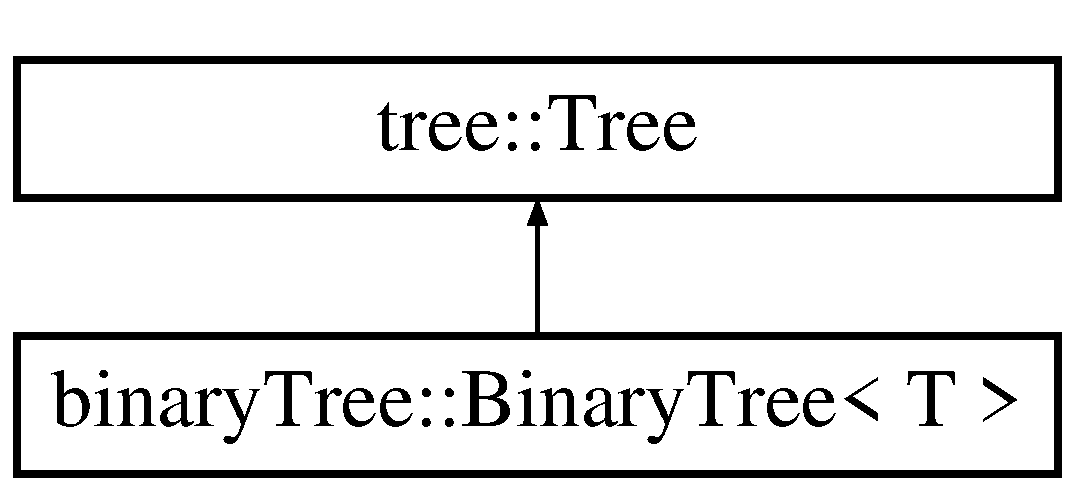
\includegraphics[height=2.000000cm]{classbinaryTree_1_1BinaryTree}
\end{center}
\end{figure}
\subsection*{Public Member Functions}
\begin{DoxyCompactItemize}
\item 
\hyperlink{classbinaryTree_1_1BinaryTree_a0605077da9009bf1c5ce15ccdd86d4d7}{Binary\-Tree} ()
\begin{DoxyCompactList}\small\item\em Default constructor. \end{DoxyCompactList}\item 
\hyperlink{classbinaryTree_1_1BinaryTree_a4d0e855e44b6e456659d627c34e4dc8a}{$\sim$\-Binary\-Tree} ()
\begin{DoxyCompactList}\small\item\em Deconstructor. \end{DoxyCompactList}\item 
void \hyperlink{classbinaryTree_1_1BinaryTree_a0a316ce96471e890d341b792bd35818a}{insert} (T given\-Data)
\begin{DoxyCompactList}\small\item\em Insert item. \end{DoxyCompactList}\item 
void \hyperlink{classbinaryTree_1_1BinaryTree_a1c1ae9d052062a790425537d6a10b0b8}{insert} (T given\-Data, \hyperlink{structbinaryTree_1_1Node}{Node}$<$ T $>$ $\ast$given\-Node)
\begin{DoxyCompactList}\small\item\em Insert item at node. \end{DoxyCompactList}\item 
void \hyperlink{classbinaryTree_1_1BinaryTree_aab6c8ba38982c02ec902b24b76d4d167}{remove} (T given\-Data)
\begin{DoxyCompactList}\small\item\em Remove item. \end{DoxyCompactList}\item 
void \hyperlink{classbinaryTree_1_1BinaryTree_a7284bf49d7fe7b3c1e4a3541f38cd9b1}{remove} (T given\-Data, \hyperlink{structbinaryTree_1_1Node}{Node}$<$ T $>$ $\ast$given\-Node)
\begin{DoxyCompactList}\small\item\em Remove item at node. \end{DoxyCompactList}\item 
void \hyperlink{classbinaryTree_1_1BinaryTree_ad26019df7707ec33825e165e3e592fd3}{pre\-Order\-Traversal} ()
\begin{DoxyCompactList}\small\item\em pre\-Order\-Travesal from the root node \end{DoxyCompactList}\item 
void \hyperlink{classbinaryTree_1_1BinaryTree_af7c8afc9eed5189283b8b188195eb171}{pre\-Order\-Traversal} (\hyperlink{structbinaryTree_1_1Node}{Node}$<$ T $>$ $\ast$given\-Node)
\begin{DoxyCompactList}\small\item\em pre\-Order\-Travesal from a given node \end{DoxyCompactList}\item 
void \hyperlink{classbinaryTree_1_1BinaryTree_ac698ef815ef2070b9cef00da006f1499}{in\-Order\-Traversal} ()
\begin{DoxyCompactList}\small\item\em in\-Order\-Traversal from the root node \end{DoxyCompactList}\item 
void \hyperlink{classbinaryTree_1_1BinaryTree_a45ad89139b915b0c24d0e2ac812b545b}{in\-Order\-Traversal} (\hyperlink{structbinaryTree_1_1Node}{Node}$<$ T $>$ $\ast$given\-Node)
\begin{DoxyCompactList}\small\item\em in\-Order\-Traversal from a given node \end{DoxyCompactList}\item 
void \hyperlink{classbinaryTree_1_1BinaryTree_a253ebeb47bc56d441b7f58b83fed182d}{post\-Order\-Traversal} ()
\begin{DoxyCompactList}\small\item\em post\-Order\-Traversal from the root node \end{DoxyCompactList}\item 
void \hyperlink{classbinaryTree_1_1BinaryTree_a48de4d016b00cde76da6a8773eee5e52}{post\-Order\-Traversal} (\hyperlink{structbinaryTree_1_1Node}{Node}$<$ T $>$ $\ast$given\-Node)
\begin{DoxyCompactList}\small\item\em post\-Order\-Traversal from a given node \end{DoxyCompactList}\item 
void \hyperlink{classbinaryTree_1_1BinaryTree_a70a4c6b978b21172d25e4bad214bc901}{breadth\-First\-Traversal} ()
\begin{DoxyCompactList}\small\item\em breadth\-First\-Traversal from the root node \end{DoxyCompactList}\item 
void \hyperlink{classbinaryTree_1_1BinaryTree_ae18f2e99a100b60ca68c7d85563e6676}{breadth\-First\-Traversal} (\hyperlink{structbinaryTree_1_1Node}{Node}$<$ T $>$ $\ast$given\-Node)
\begin{DoxyCompactList}\small\item\em breadth\-First\-Traversal from a given node \end{DoxyCompactList}\item 
void \hyperlink{classbinaryTree_1_1BinaryTree_ad57b6b69f944ae45262c635fb7cc3bdc}{print} ()
\begin{DoxyCompactList}\small\item\em Print Binary Tree. \end{DoxyCompactList}\end{DoxyCompactItemize}
\subsection*{Protected Attributes}
\begin{DoxyCompactItemize}
\item 
int \hyperlink{classtree_1_1Tree_ae808b4b4b204faaa40e1e636ebfab8e6}{depth}
\begin{DoxyCompactList}\small\item\em \hyperlink{classtree_1_1Tree}{Tree} Depth. \end{DoxyCompactList}\end{DoxyCompactItemize}
\subsection*{Private Attributes}
\begin{DoxyCompactItemize}
\item 
\hyperlink{structbinaryTree_1_1Node}{Node}$<$ T $>$ $\ast$ \hyperlink{classbinaryTree_1_1BinaryTree_a4acdb7e36855c68a15a315ece7b6a6d3}{root}
\begin{DoxyCompactList}\small\item\em Root \hyperlink{structbinaryTree_1_1Node}{Node}. \end{DoxyCompactList}\end{DoxyCompactItemize}


\subsection{Detailed Description}
\subsubsection*{template$<$typename T$>$class binary\-Tree\-::\-Binary\-Tree$<$ T $>$}

Binary Tree class. 

Definition at line 51 of file Binary\-Tree.\-hpp.



\subsection{Constructor \& Destructor Documentation}
\hypertarget{classbinaryTree_1_1BinaryTree_a0605077da9009bf1c5ce15ccdd86d4d7}{\index{binary\-Tree\-::\-Binary\-Tree@{binary\-Tree\-::\-Binary\-Tree}!Binary\-Tree@{Binary\-Tree}}
\index{Binary\-Tree@{Binary\-Tree}!binaryTree::BinaryTree@{binary\-Tree\-::\-Binary\-Tree}}
\subsubsection[{Binary\-Tree}]{\setlength{\rightskip}{0pt plus 5cm}template$<$typename T $>$ {\bf binary\-Tree\-::\-Binary\-Tree}$<$ T $>$\-::{\bf Binary\-Tree} (
\begin{DoxyParamCaption}
{}
\end{DoxyParamCaption}
)}}\label{classbinaryTree_1_1BinaryTree_a0605077da9009bf1c5ce15ccdd86d4d7}


Default constructor. 



Definition at line 106 of file Binary\-Tree.\-hpp.

\hypertarget{classbinaryTree_1_1BinaryTree_a4d0e855e44b6e456659d627c34e4dc8a}{\index{binary\-Tree\-::\-Binary\-Tree@{binary\-Tree\-::\-Binary\-Tree}!$\sim$\-Binary\-Tree@{$\sim$\-Binary\-Tree}}
\index{$\sim$\-Binary\-Tree@{$\sim$\-Binary\-Tree}!binaryTree::BinaryTree@{binary\-Tree\-::\-Binary\-Tree}}
\subsubsection[{$\sim$\-Binary\-Tree}]{\setlength{\rightskip}{0pt plus 5cm}template$<$typename T $>$ {\bf binary\-Tree\-::\-Binary\-Tree}$<$ T $>$\-::$\sim${\bf Binary\-Tree} (
\begin{DoxyParamCaption}
{}
\end{DoxyParamCaption}
)}}\label{classbinaryTree_1_1BinaryTree_a4d0e855e44b6e456659d627c34e4dc8a}


Deconstructor. 



Definition at line 112 of file Binary\-Tree.\-hpp.



\subsection{Member Function Documentation}
\hypertarget{classbinaryTree_1_1BinaryTree_a70a4c6b978b21172d25e4bad214bc901}{\index{binary\-Tree\-::\-Binary\-Tree@{binary\-Tree\-::\-Binary\-Tree}!breadth\-First\-Traversal@{breadth\-First\-Traversal}}
\index{breadth\-First\-Traversal@{breadth\-First\-Traversal}!binaryTree::BinaryTree@{binary\-Tree\-::\-Binary\-Tree}}
\subsubsection[{breadth\-First\-Traversal}]{\setlength{\rightskip}{0pt plus 5cm}template$<$typename T $>$ void {\bf binary\-Tree\-::\-Binary\-Tree}$<$ T $>$\-::breadth\-First\-Traversal (
\begin{DoxyParamCaption}
{}
\end{DoxyParamCaption}
)}}\label{classbinaryTree_1_1BinaryTree_a70a4c6b978b21172d25e4bad214bc901}


breadth\-First\-Traversal from the root node 



Definition at line 251 of file Binary\-Tree.\-hpp.

\hypertarget{classbinaryTree_1_1BinaryTree_ae18f2e99a100b60ca68c7d85563e6676}{\index{binary\-Tree\-::\-Binary\-Tree@{binary\-Tree\-::\-Binary\-Tree}!breadth\-First\-Traversal@{breadth\-First\-Traversal}}
\index{breadth\-First\-Traversal@{breadth\-First\-Traversal}!binaryTree::BinaryTree@{binary\-Tree\-::\-Binary\-Tree}}
\subsubsection[{breadth\-First\-Traversal}]{\setlength{\rightskip}{0pt plus 5cm}template$<$typename T $>$ void {\bf binary\-Tree\-::\-Binary\-Tree}$<$ T $>$\-::breadth\-First\-Traversal (
\begin{DoxyParamCaption}
\item[{{\bf Node}$<$ T $>$ $\ast$}]{given\-Node}
\end{DoxyParamCaption}
)}}\label{classbinaryTree_1_1BinaryTree_ae18f2e99a100b60ca68c7d85563e6676}


breadth\-First\-Traversal from a given node 



Definition at line 257 of file Binary\-Tree.\-hpp.

\hypertarget{classbinaryTree_1_1BinaryTree_ac698ef815ef2070b9cef00da006f1499}{\index{binary\-Tree\-::\-Binary\-Tree@{binary\-Tree\-::\-Binary\-Tree}!in\-Order\-Traversal@{in\-Order\-Traversal}}
\index{in\-Order\-Traversal@{in\-Order\-Traversal}!binaryTree::BinaryTree@{binary\-Tree\-::\-Binary\-Tree}}
\subsubsection[{in\-Order\-Traversal}]{\setlength{\rightskip}{0pt plus 5cm}template$<$typename T $>$ void {\bf binary\-Tree\-::\-Binary\-Tree}$<$ T $>$\-::in\-Order\-Traversal (
\begin{DoxyParamCaption}
{}
\end{DoxyParamCaption}
)}}\label{classbinaryTree_1_1BinaryTree_ac698ef815ef2070b9cef00da006f1499}


in\-Order\-Traversal from the root node 



Definition at line 204 of file Binary\-Tree.\-hpp.

\hypertarget{classbinaryTree_1_1BinaryTree_a45ad89139b915b0c24d0e2ac812b545b}{\index{binary\-Tree\-::\-Binary\-Tree@{binary\-Tree\-::\-Binary\-Tree}!in\-Order\-Traversal@{in\-Order\-Traversal}}
\index{in\-Order\-Traversal@{in\-Order\-Traversal}!binaryTree::BinaryTree@{binary\-Tree\-::\-Binary\-Tree}}
\subsubsection[{in\-Order\-Traversal}]{\setlength{\rightskip}{0pt plus 5cm}template$<$typename T $>$ void {\bf binary\-Tree\-::\-Binary\-Tree}$<$ T $>$\-::in\-Order\-Traversal (
\begin{DoxyParamCaption}
\item[{{\bf Node}$<$ T $>$ $\ast$}]{given\-Node}
\end{DoxyParamCaption}
)}}\label{classbinaryTree_1_1BinaryTree_a45ad89139b915b0c24d0e2ac812b545b}


in\-Order\-Traversal from a given node 



Definition at line 210 of file Binary\-Tree.\-hpp.



References binary\-Tree\-::\-Node$<$ T $>$\-::datum, binary\-Tree\-::\-Node$<$ T $>$\-::left\-Child, and binary\-Tree\-::\-Node$<$ T $>$\-::right\-Child.

\hypertarget{classbinaryTree_1_1BinaryTree_a0a316ce96471e890d341b792bd35818a}{\index{binary\-Tree\-::\-Binary\-Tree@{binary\-Tree\-::\-Binary\-Tree}!insert@{insert}}
\index{insert@{insert}!binaryTree::BinaryTree@{binary\-Tree\-::\-Binary\-Tree}}
\subsubsection[{insert}]{\setlength{\rightskip}{0pt plus 5cm}template$<$typename T $>$ void {\bf binary\-Tree\-::\-Binary\-Tree}$<$ T $>$\-::insert (
\begin{DoxyParamCaption}
\item[{T}]{given\-Data}
\end{DoxyParamCaption}
)}}\label{classbinaryTree_1_1BinaryTree_a0a316ce96471e890d341b792bd35818a}


Insert item. 



Definition at line 117 of file Binary\-Tree.\-hpp.



References binary\-Tree\-::\-Node$<$ T $>$\-::datum.

\hypertarget{classbinaryTree_1_1BinaryTree_a1c1ae9d052062a790425537d6a10b0b8}{\index{binary\-Tree\-::\-Binary\-Tree@{binary\-Tree\-::\-Binary\-Tree}!insert@{insert}}
\index{insert@{insert}!binaryTree::BinaryTree@{binary\-Tree\-::\-Binary\-Tree}}
\subsubsection[{insert}]{\setlength{\rightskip}{0pt plus 5cm}template$<$typename T $>$ void {\bf binary\-Tree\-::\-Binary\-Tree}$<$ T $>$\-::insert (
\begin{DoxyParamCaption}
\item[{T}]{given\-Data, }
\item[{{\bf Node}$<$ T $>$ $\ast$}]{given\-Node}
\end{DoxyParamCaption}
)}}\label{classbinaryTree_1_1BinaryTree_a1c1ae9d052062a790425537d6a10b0b8}


Insert item at node. 



Definition at line 133 of file Binary\-Tree.\-hpp.



References binary\-Tree\-::\-Node$<$ T $>$\-::datum, binary\-Tree\-::\-Node$<$ T $>$\-::left\-Child, and binary\-Tree\-::\-Node$<$ T $>$\-::right\-Child.

\hypertarget{classbinaryTree_1_1BinaryTree_a253ebeb47bc56d441b7f58b83fed182d}{\index{binary\-Tree\-::\-Binary\-Tree@{binary\-Tree\-::\-Binary\-Tree}!post\-Order\-Traversal@{post\-Order\-Traversal}}
\index{post\-Order\-Traversal@{post\-Order\-Traversal}!binaryTree::BinaryTree@{binary\-Tree\-::\-Binary\-Tree}}
\subsubsection[{post\-Order\-Traversal}]{\setlength{\rightskip}{0pt plus 5cm}template$<$typename T $>$ void {\bf binary\-Tree\-::\-Binary\-Tree}$<$ T $>$\-::post\-Order\-Traversal (
\begin{DoxyParamCaption}
{}
\end{DoxyParamCaption}
)}}\label{classbinaryTree_1_1BinaryTree_a253ebeb47bc56d441b7f58b83fed182d}


post\-Order\-Traversal from the root node 



Definition at line 228 of file Binary\-Tree.\-hpp.

\hypertarget{classbinaryTree_1_1BinaryTree_a48de4d016b00cde76da6a8773eee5e52}{\index{binary\-Tree\-::\-Binary\-Tree@{binary\-Tree\-::\-Binary\-Tree}!post\-Order\-Traversal@{post\-Order\-Traversal}}
\index{post\-Order\-Traversal@{post\-Order\-Traversal}!binaryTree::BinaryTree@{binary\-Tree\-::\-Binary\-Tree}}
\subsubsection[{post\-Order\-Traversal}]{\setlength{\rightskip}{0pt plus 5cm}template$<$typename T $>$ void {\bf binary\-Tree\-::\-Binary\-Tree}$<$ T $>$\-::post\-Order\-Traversal (
\begin{DoxyParamCaption}
\item[{{\bf Node}$<$ T $>$ $\ast$}]{given\-Node}
\end{DoxyParamCaption}
)}}\label{classbinaryTree_1_1BinaryTree_a48de4d016b00cde76da6a8773eee5e52}


post\-Order\-Traversal from a given node 



Definition at line 234 of file Binary\-Tree.\-hpp.



References binary\-Tree\-::\-Node$<$ T $>$\-::datum, binary\-Tree\-::\-Node$<$ T $>$\-::left\-Child, and binary\-Tree\-::\-Node$<$ T $>$\-::right\-Child.

\hypertarget{classbinaryTree_1_1BinaryTree_ad26019df7707ec33825e165e3e592fd3}{\index{binary\-Tree\-::\-Binary\-Tree@{binary\-Tree\-::\-Binary\-Tree}!pre\-Order\-Traversal@{pre\-Order\-Traversal}}
\index{pre\-Order\-Traversal@{pre\-Order\-Traversal}!binaryTree::BinaryTree@{binary\-Tree\-::\-Binary\-Tree}}
\subsubsection[{pre\-Order\-Traversal}]{\setlength{\rightskip}{0pt plus 5cm}template$<$typename T $>$ void {\bf binary\-Tree\-::\-Binary\-Tree}$<$ T $>$\-::pre\-Order\-Traversal (
\begin{DoxyParamCaption}
{}
\end{DoxyParamCaption}
)}}\label{classbinaryTree_1_1BinaryTree_ad26019df7707ec33825e165e3e592fd3}


pre\-Order\-Travesal from the root node 



Definition at line 181 of file Binary\-Tree.\-hpp.

\hypertarget{classbinaryTree_1_1BinaryTree_af7c8afc9eed5189283b8b188195eb171}{\index{binary\-Tree\-::\-Binary\-Tree@{binary\-Tree\-::\-Binary\-Tree}!pre\-Order\-Traversal@{pre\-Order\-Traversal}}
\index{pre\-Order\-Traversal@{pre\-Order\-Traversal}!binaryTree::BinaryTree@{binary\-Tree\-::\-Binary\-Tree}}
\subsubsection[{pre\-Order\-Traversal}]{\setlength{\rightskip}{0pt plus 5cm}template$<$typename T $>$ void {\bf binary\-Tree\-::\-Binary\-Tree}$<$ T $>$\-::pre\-Order\-Traversal (
\begin{DoxyParamCaption}
\item[{{\bf Node}$<$ T $>$ $\ast$}]{given\-Node}
\end{DoxyParamCaption}
)}}\label{classbinaryTree_1_1BinaryTree_af7c8afc9eed5189283b8b188195eb171}


pre\-Order\-Travesal from a given node 



Definition at line 187 of file Binary\-Tree.\-hpp.



References binary\-Tree\-::\-Node$<$ T $>$\-::datum, binary\-Tree\-::\-Node$<$ T $>$\-::left\-Child, and binary\-Tree\-::\-Node$<$ T $>$\-::right\-Child.

\hypertarget{classbinaryTree_1_1BinaryTree_ad57b6b69f944ae45262c635fb7cc3bdc}{\index{binary\-Tree\-::\-Binary\-Tree@{binary\-Tree\-::\-Binary\-Tree}!print@{print}}
\index{print@{print}!binaryTree::BinaryTree@{binary\-Tree\-::\-Binary\-Tree}}
\subsubsection[{print}]{\setlength{\rightskip}{0pt plus 5cm}template$<$typename T $>$ void {\bf binary\-Tree\-::\-Binary\-Tree}$<$ T $>$\-::print (
\begin{DoxyParamCaption}
{}
\end{DoxyParamCaption}
)\hspace{0.3cm}{\ttfamily [virtual]}}}\label{classbinaryTree_1_1BinaryTree_ad57b6b69f944ae45262c635fb7cc3bdc}


Print Binary Tree. 



Implements \hyperlink{classtree_1_1Tree_ae5b70de2d45be21d9b1b272c945b6248}{tree\-::\-Tree}.



Definition at line 265 of file Binary\-Tree.\-hpp.

\hypertarget{classbinaryTree_1_1BinaryTree_aab6c8ba38982c02ec902b24b76d4d167}{\index{binary\-Tree\-::\-Binary\-Tree@{binary\-Tree\-::\-Binary\-Tree}!remove@{remove}}
\index{remove@{remove}!binaryTree::BinaryTree@{binary\-Tree\-::\-Binary\-Tree}}
\subsubsection[{remove}]{\setlength{\rightskip}{0pt plus 5cm}template$<$typename T $>$ void {\bf binary\-Tree\-::\-Binary\-Tree}$<$ T $>$\-::remove (
\begin{DoxyParamCaption}
\item[{T}]{given\-Data}
\end{DoxyParamCaption}
)}}\label{classbinaryTree_1_1BinaryTree_aab6c8ba38982c02ec902b24b76d4d167}


Remove item. 



Definition at line 169 of file Binary\-Tree.\-hpp.

\hypertarget{classbinaryTree_1_1BinaryTree_a7284bf49d7fe7b3c1e4a3541f38cd9b1}{\index{binary\-Tree\-::\-Binary\-Tree@{binary\-Tree\-::\-Binary\-Tree}!remove@{remove}}
\index{remove@{remove}!binaryTree::BinaryTree@{binary\-Tree\-::\-Binary\-Tree}}
\subsubsection[{remove}]{\setlength{\rightskip}{0pt plus 5cm}template$<$typename T $>$ void {\bf binary\-Tree\-::\-Binary\-Tree}$<$ T $>$\-::remove (
\begin{DoxyParamCaption}
\item[{T}]{given\-Data, }
\item[{{\bf Node}$<$ T $>$ $\ast$}]{given\-Node}
\end{DoxyParamCaption}
)}}\label{classbinaryTree_1_1BinaryTree_a7284bf49d7fe7b3c1e4a3541f38cd9b1}


Remove item at node. 



Definition at line 175 of file Binary\-Tree.\-hpp.



\subsection{Member Data Documentation}
\hypertarget{classtree_1_1Tree_ae808b4b4b204faaa40e1e636ebfab8e6}{\index{binary\-Tree\-::\-Binary\-Tree@{binary\-Tree\-::\-Binary\-Tree}!depth@{depth}}
\index{depth@{depth}!binaryTree::BinaryTree@{binary\-Tree\-::\-Binary\-Tree}}
\subsubsection[{depth}]{\setlength{\rightskip}{0pt plus 5cm}int tree\-::\-Tree\-::depth\hspace{0.3cm}{\ttfamily [protected]}, {\ttfamily [inherited]}}}\label{classtree_1_1Tree_ae808b4b4b204faaa40e1e636ebfab8e6}


\hyperlink{classtree_1_1Tree}{Tree} Depth. 



Definition at line 46 of file Tree.\-hpp.

\hypertarget{classbinaryTree_1_1BinaryTree_a4acdb7e36855c68a15a315ece7b6a6d3}{\index{binary\-Tree\-::\-Binary\-Tree@{binary\-Tree\-::\-Binary\-Tree}!root@{root}}
\index{root@{root}!binaryTree::BinaryTree@{binary\-Tree\-::\-Binary\-Tree}}
\subsubsection[{root}]{\setlength{\rightskip}{0pt plus 5cm}template$<$typename T $>$ {\bf Node}$<$T$>$$\ast$ {\bf binary\-Tree\-::\-Binary\-Tree}$<$ T $>$\-::root\hspace{0.3cm}{\ttfamily [private]}}}\label{classbinaryTree_1_1BinaryTree_a4acdb7e36855c68a15a315ece7b6a6d3}


Root \hyperlink{structbinaryTree_1_1Node}{Node}. 



Definition at line 55 of file Binary\-Tree.\-hpp.



The documentation for this class was generated from the following file\-:\begin{DoxyCompactItemize}
\item 
lib/\-Data\-Structures/\hyperlink{BinaryTree_8hpp}{Binary\-Tree.\-hpp}\end{DoxyCompactItemize}

\hypertarget{classBogoSort}{\section{Bogo\-Sort$<$ T $>$ Class Template Reference}
\label{classBogoSort}\index{Bogo\-Sort$<$ T $>$@{Bogo\-Sort$<$ T $>$}}
}


{\ttfamily \#include \char`\"{}Bogo\-Sort.\-hpp\char`\"{}}

\subsection*{Public Member Functions}
\begin{DoxyCompactItemize}
\item 
\hyperlink{classBogoSort_a70d62ac6e535c9768925b76557420e9d}{Bogo\-Sort} ()
\item 
\hyperlink{classBogoSort_af3f2da4dfd2c346c9ee1a6faf5e34eb0}{Bogo\-Sort} (std\-::vector$<$ T $>$ in\-List)
\item 
int \hyperlink{classBogoSort_a3df736ca0fbf29887e2d18de3baf6dca}{sort} ()
\item 
void \hyperlink{classBogoSort_a94fdf878f8e80e93f1e3c65a41c3f4a3}{print} ()
\end{DoxyCompactItemize}
\subsection*{Private Attributes}
\begin{DoxyCompactItemize}
\item 
std\-::vector$<$ T $>$ \hyperlink{classBogoSort_ae72e81578cb2ad4e7122022d2dfffba8}{list}
\end{DoxyCompactItemize}


\subsection{Detailed Description}
\subsubsection*{template$<$typename T$>$class Bogo\-Sort$<$ T $>$}



Definition at line 31 of file Bogo\-Sort.\-hpp.



\subsection{Constructor \& Destructor Documentation}
\hypertarget{classBogoSort_a70d62ac6e535c9768925b76557420e9d}{\index{Bogo\-Sort@{Bogo\-Sort}!Bogo\-Sort@{Bogo\-Sort}}
\index{Bogo\-Sort@{Bogo\-Sort}!BogoSort@{Bogo\-Sort}}
\subsubsection[{Bogo\-Sort}]{\setlength{\rightskip}{0pt plus 5cm}template$<$typename T $>$ {\bf Bogo\-Sort}$<$ T $>$\-::{\bf Bogo\-Sort} (
\begin{DoxyParamCaption}
{}
\end{DoxyParamCaption}
)}}\label{classBogoSort_a70d62ac6e535c9768925b76557420e9d}


Definition at line 47 of file Bogo\-Sort.\-hpp.

\hypertarget{classBogoSort_af3f2da4dfd2c346c9ee1a6faf5e34eb0}{\index{Bogo\-Sort@{Bogo\-Sort}!Bogo\-Sort@{Bogo\-Sort}}
\index{Bogo\-Sort@{Bogo\-Sort}!BogoSort@{Bogo\-Sort}}
\subsubsection[{Bogo\-Sort}]{\setlength{\rightskip}{0pt plus 5cm}template$<$typename T $>$ {\bf Bogo\-Sort}$<$ T $>$\-::{\bf Bogo\-Sort} (
\begin{DoxyParamCaption}
\item[{std\-::vector$<$ T $>$}]{in\-List}
\end{DoxyParamCaption}
)}}\label{classBogoSort_af3f2da4dfd2c346c9ee1a6faf5e34eb0}


Definition at line 53 of file Bogo\-Sort.\-hpp.



\subsection{Member Function Documentation}
\hypertarget{classBogoSort_a94fdf878f8e80e93f1e3c65a41c3f4a3}{\index{Bogo\-Sort@{Bogo\-Sort}!print@{print}}
\index{print@{print}!BogoSort@{Bogo\-Sort}}
\subsubsection[{print}]{\setlength{\rightskip}{0pt plus 5cm}template$<$typename T $>$ void {\bf Bogo\-Sort}$<$ T $>$\-::print (
\begin{DoxyParamCaption}
{}
\end{DoxyParamCaption}
)}}\label{classBogoSort_a94fdf878f8e80e93f1e3c65a41c3f4a3}


Definition at line 76 of file Bogo\-Sort.\-hpp.

\hypertarget{classBogoSort_a3df736ca0fbf29887e2d18de3baf6dca}{\index{Bogo\-Sort@{Bogo\-Sort}!sort@{sort}}
\index{sort@{sort}!BogoSort@{Bogo\-Sort}}
\subsubsection[{sort}]{\setlength{\rightskip}{0pt plus 5cm}template$<$typename T $>$ int {\bf Bogo\-Sort}$<$ T $>$\-::sort (
\begin{DoxyParamCaption}
{}
\end{DoxyParamCaption}
)}}\label{classBogoSort_a3df736ca0fbf29887e2d18de3baf6dca}


Definition at line 59 of file Bogo\-Sort.\-hpp.



\subsection{Member Data Documentation}
\hypertarget{classBogoSort_ae72e81578cb2ad4e7122022d2dfffba8}{\index{Bogo\-Sort@{Bogo\-Sort}!list@{list}}
\index{list@{list}!BogoSort@{Bogo\-Sort}}
\subsubsection[{list}]{\setlength{\rightskip}{0pt plus 5cm}template$<$typename T $>$ std\-::vector$<$T$>$ {\bf Bogo\-Sort}$<$ T $>$\-::list\hspace{0.3cm}{\ttfamily [private]}}}\label{classBogoSort_ae72e81578cb2ad4e7122022d2dfffba8}


Definition at line 34 of file Bogo\-Sort.\-hpp.



The documentation for this class was generated from the following file\-:\begin{DoxyCompactItemize}
\item 
lib/\-Sorting/\hyperlink{BogoSort_8hpp}{Bogo\-Sort.\-hpp}\end{DoxyCompactItemize}

\hypertarget{classdoublyLinkedList_1_1DoublyLinkedList}{\section{doubly\-Linked\-List\-:\-:Doubly\-Linked\-List$<$ T $>$ Class Template Reference}
\label{classdoublyLinkedList_1_1DoublyLinkedList}\index{doubly\-Linked\-List\-::\-Doubly\-Linked\-List$<$ T $>$@{doubly\-Linked\-List\-::\-Doubly\-Linked\-List$<$ T $>$}}
}


{\ttfamily \#include \char`\"{}Doubly\-Linked\-List.\-hpp\char`\"{}}

\subsection*{Public Member Functions}
\begin{DoxyCompactItemize}
\item 
\hyperlink{classdoublyLinkedList_1_1DoublyLinkedList_a2b10fc07de33dbdc2fa37c1765c52946}{Doubly\-Linked\-List} ()
\item 
void \hyperlink{classdoublyLinkedList_1_1DoublyLinkedList_aaecb4b25b712cf777f20de65c87b0629}{push\-Back} (T data)
\item 
void \hyperlink{classdoublyLinkedList_1_1DoublyLinkedList_a4170c12e58db34d356225a05bb9684f1}{push\-Front} (T data)
\item 
void \hyperlink{classdoublyLinkedList_1_1DoublyLinkedList_a53d85f48953602617330b8abdd6efa5b}{pop\-Back} (T data)
\item 
void \hyperlink{classdoublyLinkedList_1_1DoublyLinkedList_ad6714a20e69f0b31d943963b57f563e2}{pop\-Front} (T data)
\item 
void \hyperlink{classdoublyLinkedList_1_1DoublyLinkedList_a61e3cc34cd060e6ed80761cc226f3da5}{print} ()
\end{DoxyCompactItemize}
\subsection*{Private Attributes}
\begin{DoxyCompactItemize}
\item 
\hyperlink{structdoublyLinkedList_1_1Node}{Node}$<$ T $>$ $\ast$ \hyperlink{classdoublyLinkedList_1_1DoublyLinkedList_ab29d146595ee66d859611599bbccc19d}{head}
\item 
\hyperlink{structdoublyLinkedList_1_1Node}{Node}$<$ T $>$ $\ast$ \hyperlink{classdoublyLinkedList_1_1DoublyLinkedList_af31f560be2e8532064d74d1c2466a114}{tail}
\item 
int \hyperlink{classdoublyLinkedList_1_1DoublyLinkedList_a894259d7ab4a0e16bf3a1221d1d4bc75}{size}
\end{DoxyCompactItemize}


\subsection{Detailed Description}
\subsubsection*{template$<$typename T$>$class doubly\-Linked\-List\-::\-Doubly\-Linked\-List$<$ T $>$}



Definition at line 40 of file Doubly\-Linked\-List.\-hpp.



\subsection{Constructor \& Destructor Documentation}
\hypertarget{classdoublyLinkedList_1_1DoublyLinkedList_a2b10fc07de33dbdc2fa37c1765c52946}{\index{doubly\-Linked\-List\-::\-Doubly\-Linked\-List@{doubly\-Linked\-List\-::\-Doubly\-Linked\-List}!Doubly\-Linked\-List@{Doubly\-Linked\-List}}
\index{Doubly\-Linked\-List@{Doubly\-Linked\-List}!doublyLinkedList::DoublyLinkedList@{doubly\-Linked\-List\-::\-Doubly\-Linked\-List}}
\subsubsection[{Doubly\-Linked\-List}]{\setlength{\rightskip}{0pt plus 5cm}template$<$typename T $>$ {\bf doubly\-Linked\-List\-::\-Doubly\-Linked\-List}$<$ T $>$\-::{\bf Doubly\-Linked\-List} (
\begin{DoxyParamCaption}
{}
\end{DoxyParamCaption}
)}}\label{classdoublyLinkedList_1_1DoublyLinkedList_a2b10fc07de33dbdc2fa37c1765c52946}


Definition at line 63 of file Doubly\-Linked\-List.\-hpp.



\subsection{Member Function Documentation}
\hypertarget{classdoublyLinkedList_1_1DoublyLinkedList_a53d85f48953602617330b8abdd6efa5b}{\index{doubly\-Linked\-List\-::\-Doubly\-Linked\-List@{doubly\-Linked\-List\-::\-Doubly\-Linked\-List}!pop\-Back@{pop\-Back}}
\index{pop\-Back@{pop\-Back}!doublyLinkedList::DoublyLinkedList@{doubly\-Linked\-List\-::\-Doubly\-Linked\-List}}
\subsubsection[{pop\-Back}]{\setlength{\rightskip}{0pt plus 5cm}template$<$typename T $>$ void {\bf doubly\-Linked\-List\-::\-Doubly\-Linked\-List}$<$ T $>$\-::pop\-Back (
\begin{DoxyParamCaption}
\item[{T}]{data}
\end{DoxyParamCaption}
)}}\label{classdoublyLinkedList_1_1DoublyLinkedList_a53d85f48953602617330b8abdd6efa5b}


Definition at line 104 of file Doubly\-Linked\-List.\-hpp.



References doubly\-Linked\-List\-::\-Node$<$ T $>$\-::datum.

\hypertarget{classdoublyLinkedList_1_1DoublyLinkedList_ad6714a20e69f0b31d943963b57f563e2}{\index{doubly\-Linked\-List\-::\-Doubly\-Linked\-List@{doubly\-Linked\-List\-::\-Doubly\-Linked\-List}!pop\-Front@{pop\-Front}}
\index{pop\-Front@{pop\-Front}!doublyLinkedList::DoublyLinkedList@{doubly\-Linked\-List\-::\-Doubly\-Linked\-List}}
\subsubsection[{pop\-Front}]{\setlength{\rightskip}{0pt plus 5cm}template$<$typename T $>$ void {\bf doubly\-Linked\-List\-::\-Doubly\-Linked\-List}$<$ T $>$\-::pop\-Front (
\begin{DoxyParamCaption}
\item[{T}]{data}
\end{DoxyParamCaption}
)}}\label{classdoublyLinkedList_1_1DoublyLinkedList_ad6714a20e69f0b31d943963b57f563e2}


Definition at line 119 of file Doubly\-Linked\-List.\-hpp.

\hypertarget{classdoublyLinkedList_1_1DoublyLinkedList_a61e3cc34cd060e6ed80761cc226f3da5}{\index{doubly\-Linked\-List\-::\-Doubly\-Linked\-List@{doubly\-Linked\-List\-::\-Doubly\-Linked\-List}!print@{print}}
\index{print@{print}!doublyLinkedList::DoublyLinkedList@{doubly\-Linked\-List\-::\-Doubly\-Linked\-List}}
\subsubsection[{print}]{\setlength{\rightskip}{0pt plus 5cm}template$<$typename T $>$ void {\bf doubly\-Linked\-List\-::\-Doubly\-Linked\-List}$<$ T $>$\-::print (
\begin{DoxyParamCaption}
{}
\end{DoxyParamCaption}
)}}\label{classdoublyLinkedList_1_1DoublyLinkedList_a61e3cc34cd060e6ed80761cc226f3da5}


Definition at line 125 of file Doubly\-Linked\-List.\-hpp.



References doubly\-Linked\-List\-::\-Node$<$ T $>$\-::datum, and doubly\-Linked\-List\-::\-Node$<$ T $>$\-::next.

\hypertarget{classdoublyLinkedList_1_1DoublyLinkedList_aaecb4b25b712cf777f20de65c87b0629}{\index{doubly\-Linked\-List\-::\-Doubly\-Linked\-List@{doubly\-Linked\-List\-::\-Doubly\-Linked\-List}!push\-Back@{push\-Back}}
\index{push\-Back@{push\-Back}!doublyLinkedList::DoublyLinkedList@{doubly\-Linked\-List\-::\-Doubly\-Linked\-List}}
\subsubsection[{push\-Back}]{\setlength{\rightskip}{0pt plus 5cm}template$<$typename T $>$ void {\bf doubly\-Linked\-List\-::\-Doubly\-Linked\-List}$<$ T $>$\-::push\-Back (
\begin{DoxyParamCaption}
\item[{T}]{data}
\end{DoxyParamCaption}
)}}\label{classdoublyLinkedList_1_1DoublyLinkedList_aaecb4b25b712cf777f20de65c87b0629}


Definition at line 71 of file Doubly\-Linked\-List.\-hpp.



References doubly\-Linked\-List\-::\-Node$<$ T $>$\-::datum, doubly\-Linked\-List\-::\-Node$<$ T $>$\-::next, and doubly\-Linked\-List\-::\-Node$<$ T $>$\-::prev.

\hypertarget{classdoublyLinkedList_1_1DoublyLinkedList_a4170c12e58db34d356225a05bb9684f1}{\index{doubly\-Linked\-List\-::\-Doubly\-Linked\-List@{doubly\-Linked\-List\-::\-Doubly\-Linked\-List}!push\-Front@{push\-Front}}
\index{push\-Front@{push\-Front}!doublyLinkedList::DoublyLinkedList@{doubly\-Linked\-List\-::\-Doubly\-Linked\-List}}
\subsubsection[{push\-Front}]{\setlength{\rightskip}{0pt plus 5cm}template$<$typename T $>$ void {\bf doubly\-Linked\-List\-::\-Doubly\-Linked\-List}$<$ T $>$\-::push\-Front (
\begin{DoxyParamCaption}
\item[{T}]{data}
\end{DoxyParamCaption}
)}}\label{classdoublyLinkedList_1_1DoublyLinkedList_a4170c12e58db34d356225a05bb9684f1}


Definition at line 98 of file Doubly\-Linked\-List.\-hpp.



\subsection{Member Data Documentation}
\hypertarget{classdoublyLinkedList_1_1DoublyLinkedList_ab29d146595ee66d859611599bbccc19d}{\index{doubly\-Linked\-List\-::\-Doubly\-Linked\-List@{doubly\-Linked\-List\-::\-Doubly\-Linked\-List}!head@{head}}
\index{head@{head}!doublyLinkedList::DoublyLinkedList@{doubly\-Linked\-List\-::\-Doubly\-Linked\-List}}
\subsubsection[{head}]{\setlength{\rightskip}{0pt plus 5cm}template$<$typename T $>$ {\bf Node}$<$T$>$$\ast$ {\bf doubly\-Linked\-List\-::\-Doubly\-Linked\-List}$<$ T $>$\-::head\hspace{0.3cm}{\ttfamily [private]}}}\label{classdoublyLinkedList_1_1DoublyLinkedList_ab29d146595ee66d859611599bbccc19d}


Definition at line 43 of file Doubly\-Linked\-List.\-hpp.

\hypertarget{classdoublyLinkedList_1_1DoublyLinkedList_a894259d7ab4a0e16bf3a1221d1d4bc75}{\index{doubly\-Linked\-List\-::\-Doubly\-Linked\-List@{doubly\-Linked\-List\-::\-Doubly\-Linked\-List}!size@{size}}
\index{size@{size}!doublyLinkedList::DoublyLinkedList@{doubly\-Linked\-List\-::\-Doubly\-Linked\-List}}
\subsubsection[{size}]{\setlength{\rightskip}{0pt plus 5cm}template$<$typename T $>$ int {\bf doubly\-Linked\-List\-::\-Doubly\-Linked\-List}$<$ T $>$\-::size\hspace{0.3cm}{\ttfamily [private]}}}\label{classdoublyLinkedList_1_1DoublyLinkedList_a894259d7ab4a0e16bf3a1221d1d4bc75}


Definition at line 45 of file Doubly\-Linked\-List.\-hpp.

\hypertarget{classdoublyLinkedList_1_1DoublyLinkedList_af31f560be2e8532064d74d1c2466a114}{\index{doubly\-Linked\-List\-::\-Doubly\-Linked\-List@{doubly\-Linked\-List\-::\-Doubly\-Linked\-List}!tail@{tail}}
\index{tail@{tail}!doublyLinkedList::DoublyLinkedList@{doubly\-Linked\-List\-::\-Doubly\-Linked\-List}}
\subsubsection[{tail}]{\setlength{\rightskip}{0pt plus 5cm}template$<$typename T $>$ {\bf Node}$<$T$>$$\ast$ {\bf doubly\-Linked\-List\-::\-Doubly\-Linked\-List}$<$ T $>$\-::tail\hspace{0.3cm}{\ttfamily [private]}}}\label{classdoublyLinkedList_1_1DoublyLinkedList_af31f560be2e8532064d74d1c2466a114}


Definition at line 44 of file Doubly\-Linked\-List.\-hpp.



The documentation for this class was generated from the following file\-:\begin{DoxyCompactItemize}
\item 
lib/\-Data\-Structures/\hyperlink{DoublyLinkedList_8hpp}{Doubly\-Linked\-List.\-hpp}\end{DoxyCompactItemize}

\hypertarget{classmatrix_1_1Matrix}{\section{matrix\-:\-:Matrix$<$ T $>$ Class Template Reference}
\label{classmatrix_1_1Matrix}\index{matrix\-::\-Matrix$<$ T $>$@{matrix\-::\-Matrix$<$ T $>$}}
}


\hyperlink{classmatrix_1_1Matrix}{Matrix} class.  




{\ttfamily \#include \char`\"{}Matrix.\-hpp\char`\"{}}

\subsection*{Public Member Functions}
\begin{DoxyCompactItemize}
\item 
\hyperlink{classmatrix_1_1Matrix_a054d22cc5b7c78711c823310f71495f5}{Matrix} ()
\begin{DoxyCompactList}\small\item\em Default Constructor. \end{DoxyCompactList}\item 
\hyperlink{classmatrix_1_1Matrix_a2197dc025b1a32ceba87677d0d5b988d}{Matrix} (const \hyperlink{classmatrix_1_1Matrix}{Matrix}$<$ T $>$ \&rhs)
\begin{DoxyCompactList}\small\item\em Copy Constructor. \end{DoxyCompactList}\item 
\hyperlink{classmatrix_1_1Matrix_a823e33972f72b1f942099982dc101fea}{Matrix} (uint32\-\_\-t \-\_\-num\-Rows, uint32\-\_\-t \-\_\-num\-Cols, const T \&init\-Vals=0, const std\-::string \&\-\_\-pad=\hyperlink{namespacematrix_a3410a3377815b8c5431e5436a31774c4}{empty\-Str})
\begin{DoxyCompactList}\small\item\em Custom Constructor. \end{DoxyCompactList}\item 
\hyperlink{classmatrix_1_1Matrix_ab79912b5a12d7aa327e6bf0d918f4de9}{Matrix} (std\-::initializer\-\_\-list$<$ std\-::initializer\-\_\-list$<$ T $>$$>$ \-\_\-matrix)
\begin{DoxyCompactList}\small\item\em Initializer\-\_\-list Constructor. \end{DoxyCompactList}\item 
\hyperlink{classmatrix_1_1Matrix_a936cd883f1768e78478925929ea3d147}{$\sim$\-Matrix} ()
\begin{DoxyCompactList}\small\item\em Deconstructor. \end{DoxyCompactList}\item 
std\-::vector$<$ std\-::vector$<$ T $>$ $>$ \hyperlink{classmatrix_1_1Matrix_a160cd27af60a63f8ecb512f1c3ed610e}{get\-Matrix} () const 
\begin{DoxyCompactList}\small\item\em \hyperlink{classmatrix_1_1Matrix}{Matrix} Accessor. \end{DoxyCompactList}\item 
uint32\-\_\-t \hyperlink{classmatrix_1_1Matrix_a0ac23e8199500d3abecd39f5c4971149}{get\-Num\-Rows} () const 
\item 
uint32\-\_\-t \hyperlink{classmatrix_1_1Matrix_a344f628c8fc36c61da00cdd1cf9425e4}{get\-Num\-Cols} () const 
\begin{DoxyCompactList}\small\item\em Row accessor. \end{DoxyCompactList}\item 
std\-::string \hyperlink{classmatrix_1_1Matrix_ad0cc3825f9c5a88baec185be52a56af7}{get\-Pad} () const 
\begin{DoxyCompactList}\small\item\em Columns accessor. \end{DoxyCompactList}\item 
void \hyperlink{classmatrix_1_1Matrix_a83c1665465ab7ef98fa7003127cadac9}{set\-Pad} (const std\-::string \&\-\_\-pad)
\begin{DoxyCompactList}\small\item\em Pad accessor. \end{DoxyCompactList}\item 
\hyperlink{classmatrix_1_1Matrix}{Matrix}$<$ T $>$ \& \hyperlink{classmatrix_1_1Matrix_a5b1d2cf9e238f15d6e85e8084feafe83}{operator=} (const \hyperlink{classmatrix_1_1Matrix}{Matrix}$<$ T $>$ \&rhs)
\begin{DoxyCompactList}\small\item\em Assignment. \end{DoxyCompactList}\item 
\hyperlink{classmatrix_1_1Matrix}{Matrix}$<$ T $>$ \hyperlink{classmatrix_1_1Matrix_ad99f5a3971abebfe3545dde85612268f}{operator$\ast$} (const \hyperlink{classmatrix_1_1Matrix}{Matrix}$<$ T $>$ \&rhs) const 
\begin{DoxyCompactList}\small\item\em Matrix/\-Matrix Multiplication. \end{DoxyCompactList}\item 
\hyperlink{classmatrix_1_1Matrix}{Matrix}$<$ T $>$ \hyperlink{classmatrix_1_1Matrix_a62767d118083954b144767496c02205c}{operator+} (const \hyperlink{classmatrix_1_1Matrix}{Matrix}$<$ T $>$ \&rhs) const 
\begin{DoxyCompactList}\small\item\em Matrix/\-Matrix Addition. \end{DoxyCompactList}\item 
\hyperlink{classmatrix_1_1Matrix}{Matrix}$<$ T $>$ \hyperlink{classmatrix_1_1Matrix_aac28bf5632d40be2c595ccbf9bfe66a8}{operator-\/} (const \hyperlink{classmatrix_1_1Matrix}{Matrix}$<$ T $>$ \&rhs) const 
\begin{DoxyCompactList}\small\item\em Matrix/\-Matrix Subtraction. \end{DoxyCompactList}\item 
\hyperlink{classmatrix_1_1Matrix}{Matrix}$<$ T $>$ \hyperlink{classmatrix_1_1Matrix_a383ea46be492b62685a3c66b402c31d3}{operator$\ast$} (const T \&rhs) const 
\begin{DoxyCompactList}\small\item\em Matrix/\-Scalar Multiplication. \end{DoxyCompactList}\item 
\hyperlink{classmatrix_1_1Matrix}{Matrix}$<$ T $>$ \hyperlink{classmatrix_1_1Matrix_a31b5e71015aba29bd63ddb32a43aacf6}{operator/} (const T \&rhs) const 
\begin{DoxyCompactList}\small\item\em Matrix/\-Scalar Division. \end{DoxyCompactList}\item 
\hyperlink{classmatrix_1_1Matrix}{Matrix}$<$ T $>$ \hyperlink{classmatrix_1_1Matrix_a4796eea2f39bbfa3ff7f9ea4a5e5f423}{operator+} (const T \&rhs) const 
\begin{DoxyCompactList}\small\item\em Matrix/\-Scalar Addition. \end{DoxyCompactList}\item 
\hyperlink{classmatrix_1_1Matrix}{Matrix}$<$ T $>$ \hyperlink{classmatrix_1_1Matrix_ac446198a45ad411e346504c6e4698952}{operator-\/} (const T \&rhs) const 
\begin{DoxyCompactList}\small\item\em Matrix/\-Scalar Subtraction. \end{DoxyCompactList}\item 
\hyperlink{classmatrix_1_1Matrix}{Matrix}$<$ T $>$ \hyperlink{classmatrix_1_1Matrix_abc3f4492ae439d7a0791bbc4e9449cb5}{operator-\/} () const 
\begin{DoxyCompactList}\small\item\em \hyperlink{classmatrix_1_1Matrix}{Matrix} Negative. \end{DoxyCompactList}\item 
\hyperlink{classmatrix_1_1Matrix}{Matrix}$<$ T $>$ \hyperlink{classmatrix_1_1Matrix_afb301157a2f218f5877793e8a238fc58}{operator$^\wedge$} (const uint32\-\_\-t \&power) const 
\begin{DoxyCompactList}\small\item\em \hyperlink{classmatrix_1_1Matrix}{Matrix} Power function. \end{DoxyCompactList}\item 
T \& \hyperlink{classmatrix_1_1Matrix_a3512dde740a7f45fb0484ee708887444}{operator()} (const uint32\-\_\-t \&row, const uint32\-\_\-t \&col)
\begin{DoxyCompactList}\small\item\em \hyperlink{classmatrix_1_1Matrix}{Matrix} Element Access. \end{DoxyCompactList}\item 
const T \& \hyperlink{classmatrix_1_1Matrix_a02230069885fb794d62f9d544103a987}{operator()} (const uint32\-\_\-t \&row, const uint32\-\_\-t \&col) const 
\begin{DoxyCompactList}\small\item\em \hyperlink{classmatrix_1_1Matrix}{Matrix} Element Access (const) \end{DoxyCompactList}\item 
bool \hyperlink{classmatrix_1_1Matrix_ac6de29be44b19310f134cffd3328017d}{operator==} (const \hyperlink{classmatrix_1_1Matrix}{Matrix}$<$ T $>$ \&rhs) const 
\begin{DoxyCompactList}\small\item\em \hyperlink{classmatrix_1_1Matrix}{Matrix} Comparison. \end{DoxyCompactList}\item 
\hyperlink{classmatrix_1_1Matrix}{Matrix}$<$ T $>$ \hyperlink{classmatrix_1_1Matrix_ac327db77a3c97f88e2a470c1205ddabd}{transpose} () const 
\begin{DoxyCompactList}\small\item\em \hyperlink{classmatrix_1_1Matrix}{Matrix} Transpose. \end{DoxyCompactList}\item 
\hyperlink{classmatrix_1_1Matrix}{Matrix}$<$ T $>$ \hyperlink{classmatrix_1_1Matrix_a47464577950758a8a1da8455ea73ae27}{complex\-Conjugate} () const 
\begin{DoxyCompactList}\small\item\em \hyperlink{classmatrix_1_1Matrix}{Matrix} Complex Conjugate. \end{DoxyCompactList}\item 
\hyperlink{classmatrix_1_1Matrix}{Matrix}$<$ T $>$ \hyperlink{classmatrix_1_1Matrix_a93366f67006829caba19b525814596ec}{conjugate\-Transpose} () const 
\begin{DoxyCompactList}\small\item\em \hyperlink{classmatrix_1_1Matrix}{Matrix} Complex Conjugate Transpose. \end{DoxyCompactList}\item 
\hyperlink{classmatrix_1_1Matrix}{Matrix}$<$ T $>$ \hyperlink{classmatrix_1_1Matrix_a88fecb03afc587c908065bc920da5e55}{identity} () const 
\begin{DoxyCompactList}\small\item\em Identity matrix of same size and type. \end{DoxyCompactList}\item 
bool \hyperlink{classmatrix_1_1Matrix_a97d081b32df645d41eeccd7eb60464cc}{is\-Square} () const 
\begin{DoxyCompactList}\small\item\em Is matrix square? \end{DoxyCompactList}\item 
bool \hyperlink{classmatrix_1_1Matrix_a151e185fb20fcc5913cf030e172dec91}{is\-Real} () const 
\begin{DoxyCompactList}\small\item\em Are all elements real? \end{DoxyCompactList}\item 
bool \hyperlink{classmatrix_1_1Matrix_a6290d8381c92824a415850701a386572}{is\-Complex} () const 
\begin{DoxyCompactList}\small\item\em Do any elements have imaginary parts? \end{DoxyCompactList}\item 
bool \hyperlink{classmatrix_1_1Matrix_a4f327f5ad7ef829a64d0f4ef3e20d29c}{is\-Symmetric} () const 
\begin{DoxyCompactList}\small\item\em A = A$^\wedge$\-T ? \end{DoxyCompactList}\item 
bool \hyperlink{classmatrix_1_1Matrix_ad85456fb492eac300607fad58ae83b3b}{is\-Skew\-Symmetric} () const 
\begin{DoxyCompactList}\small\item\em -\/\-A = A$^\wedge$\-T ? \end{DoxyCompactList}\item 
bool \hyperlink{classmatrix_1_1Matrix_aef901991ff8a7effe565e56ddd43746e}{is\-Hermitian} () const 
\begin{DoxyCompactList}\small\item\em A = A$^\wedge$dagger (Complex extension of \hyperlink{classmatrix_1_1Matrix_a4f327f5ad7ef829a64d0f4ef3e20d29c}{is\-Symmetric()}) ? \end{DoxyCompactList}\item 
bool \hyperlink{classmatrix_1_1Matrix_a6cf8b183026095222f8385d4f5101da7}{is\-Self\-Adjoint} () const 
\begin{DoxyCompactList}\small\item\em Same as \hyperlink{classmatrix_1_1Matrix_aef901991ff8a7effe565e56ddd43746e}{is\-Hermitian()} \end{DoxyCompactList}\item 
bool \hyperlink{classmatrix_1_1Matrix_a9a68a213355b21b0de2f9893944f8655}{is\-Skew\-Hermitian} () const 
\begin{DoxyCompactList}\small\item\em -\/\-A = A$^\wedge$dagger (Complex extension of \hyperlink{classmatrix_1_1Matrix_ad85456fb492eac300607fad58ae83b3b}{is\-Skew\-Symmetric()}) \end{DoxyCompactList}\item 
bool \hyperlink{classmatrix_1_1Matrix_afe2b7f3d7e5a2cfc9201ae003609015a}{is\-Normal} () const 
\begin{DoxyCompactList}\small\item\em Real\-: A$\ast$\-A$^\wedge$\-T = A$^\wedge$\-T$\ast$\-A; Complex\-: A$\ast$\-A$^\wedge$dagger = A$^\wedge$dagger$\ast$\-A. \end{DoxyCompactList}\item 
bool \hyperlink{classmatrix_1_1Matrix_afda8e7a5303dc685cc81ccaac6aa6e98}{is\-Orthogonal} () const 
\begin{DoxyCompactList}\small\item\em A$\ast$\-A$^\wedge$\-T = A$^\wedge$\-T$\ast$\-A = I. \end{DoxyCompactList}\item 
bool \hyperlink{classmatrix_1_1Matrix_a747a89e859c3222d2fca232f2caacf4e}{is\-Unitary} () const 
\begin{DoxyCompactList}\small\item\em A$\ast$\-A$^\wedge$dagger = A$^\wedge$dagger$\ast$\-A = I (Complex extension of \hyperlink{classmatrix_1_1Matrix_afda8e7a5303dc685cc81ccaac6aa6e98}{is\-Orthogonal()}) \end{DoxyCompactList}\item 
bool \hyperlink{classmatrix_1_1Matrix_a08bab97349704f714b37ba9c27110514}{is\-Projection} () const 
\begin{DoxyCompactList}\small\item\em A = A$^\wedge$2. \end{DoxyCompactList}\item 
bool \hyperlink{classmatrix_1_1Matrix_a2ada015d14c14acedba61a68818cde59}{is\-Identity} () const 
\begin{DoxyCompactList}\small\item\em A = I. \end{DoxyCompactList}\item 
bool \hyperlink{classmatrix_1_1Matrix_ac5e3210355a0ef21cb754f0015c101ff}{commutes\-With} (const \hyperlink{classmatrix_1_1Matrix}{Matrix}$<$ T $>$ \&rhs) const 
\item 
T \hyperlink{classmatrix_1_1Matrix_a02b6c5546a65c5af50cff7a48094f312}{trace} () const 
\begin{DoxyCompactList}\small\item\em Sum of diagonal elements. \end{DoxyCompactList}\item 
T \hyperlink{classmatrix_1_1Matrix_af19c4e8032c3364ab08791e25ecccf01}{sum} () const 
\begin{DoxyCompactList}\small\item\em Sum of all elements. \end{DoxyCompactList}\end{DoxyCompactItemize}
\subsection*{Private Attributes}
\begin{DoxyCompactItemize}
\item 
std\-::vector$<$ std\-::vector$<$ T $>$ $>$ \hyperlink{classmatrix_1_1Matrix_a7d867ccf6e5f0fab0afb93b4eacefd06}{matrix}
\begin{DoxyCompactList}\small\item\em \hyperlink{classmatrix_1_1Matrix}{Matrix}. \end{DoxyCompactList}\item 
uint32\-\_\-t \hyperlink{classmatrix_1_1Matrix_ab58c595a633eaaf7ea4845cce59c90fb}{num\-Rows}
\begin{DoxyCompactList}\small\item\em Number of rows. \end{DoxyCompactList}\item 
uint32\-\_\-t \hyperlink{classmatrix_1_1Matrix_a5571a658e4320efa3312dac1081b0ce2}{num\-Cols}
\begin{DoxyCompactList}\small\item\em Number of columns. \end{DoxyCompactList}\item 
std\-::string \hyperlink{classmatrix_1_1Matrix_a361ac8fbb03f94da4b76767a747e5b71}{pad}
\begin{DoxyCompactList}\small\item\em Pad used when printing matrix. \end{DoxyCompactList}\end{DoxyCompactItemize}
\subsection*{Friends}
\begin{DoxyCompactItemize}
\item 
{\footnotesize template$<$typename U $>$ }\\std\-::ostream \& \hyperlink{classmatrix_1_1Matrix_a44e735ed3a255c4f26f2ef273f6508ee}{operator$<$$<$} (std\-::ostream \&os, const \hyperlink{classmatrix_1_1Matrix}{Matrix}$<$ T $>$ \&rhs)
\begin{DoxyCompactList}\small\item\em Pad modifier. \end{DoxyCompactList}\end{DoxyCompactItemize}


\subsection{Detailed Description}
\subsubsection*{template$<$typename T$>$class matrix\-::\-Matrix$<$ T $>$}

\hyperlink{classmatrix_1_1Matrix}{Matrix} class. 

Definition at line 41 of file Matrix.\-hpp.



\subsection{Constructor \& Destructor Documentation}
\hypertarget{classmatrix_1_1Matrix_a054d22cc5b7c78711c823310f71495f5}{\index{matrix\-::\-Matrix@{matrix\-::\-Matrix}!Matrix@{Matrix}}
\index{Matrix@{Matrix}!matrix::Matrix@{matrix\-::\-Matrix}}
\subsubsection[{Matrix}]{\setlength{\rightskip}{0pt plus 5cm}template$<$typename T $>$ {\bf matrix\-::\-Matrix}$<$ T $>$\-::{\bf Matrix} (
\begin{DoxyParamCaption}
{}
\end{DoxyParamCaption}
)}}\label{classmatrix_1_1Matrix_a054d22cc5b7c78711c823310f71495f5}


Default Constructor. 



Definition at line 214 of file Matrix.\-hpp.



References matrix\-::\-Matrix$<$ T $>$\-::matrix.

\hypertarget{classmatrix_1_1Matrix_a2197dc025b1a32ceba87677d0d5b988d}{\index{matrix\-::\-Matrix@{matrix\-::\-Matrix}!Matrix@{Matrix}}
\index{Matrix@{Matrix}!matrix::Matrix@{matrix\-::\-Matrix}}
\subsubsection[{Matrix}]{\setlength{\rightskip}{0pt plus 5cm}template$<$typename T $>$ {\bf matrix\-::\-Matrix}$<$ T $>$\-::{\bf Matrix} (
\begin{DoxyParamCaption}
\item[{const {\bf Matrix}$<$ T $>$ \&}]{rhs}
\end{DoxyParamCaption}
)}}\label{classmatrix_1_1Matrix_a2197dc025b1a32ceba87677d0d5b988d}


Copy Constructor. 


\begin{DoxyParams}{Parameters}
{\em rhs} & \hyperlink{classmatrix_1_1Matrix}{Matrix} to copy from. \\
\hline
\end{DoxyParams}


Definition at line 226 of file Matrix.\-hpp.



References matrix\-::\-Matrix$<$ T $>$\-::get\-Matrix(), matrix\-::\-Matrix$<$ T $>$\-::get\-Num\-Cols(), matrix\-::\-Matrix$<$ T $>$\-::get\-Num\-Rows(), and matrix\-::\-Matrix$<$ T $>$\-::get\-Pad().

\hypertarget{classmatrix_1_1Matrix_a823e33972f72b1f942099982dc101fea}{\index{matrix\-::\-Matrix@{matrix\-::\-Matrix}!Matrix@{Matrix}}
\index{Matrix@{Matrix}!matrix::Matrix@{matrix\-::\-Matrix}}
\subsubsection[{Matrix}]{\setlength{\rightskip}{0pt plus 5cm}template$<$typename T $>$ {\bf matrix\-::\-Matrix}$<$ T $>$\-::{\bf Matrix} (
\begin{DoxyParamCaption}
\item[{uint32\-\_\-t}]{\-\_\-num\-Rows, }
\item[{uint32\-\_\-t}]{\-\_\-num\-Cols, }
\item[{const T \&}]{init\-Vals = {\ttfamily 0}, }
\item[{const std\-::string \&}]{\-\_\-pad = {\ttfamily {\bf empty\-Str}}}
\end{DoxyParamCaption}
)}}\label{classmatrix_1_1Matrix_a823e33972f72b1f942099982dc101fea}


Custom Constructor. 


\begin{DoxyParams}{Parameters}
{\em \-\_\-num\-Rows} & Number of rows new matrix will have. \\
\hline
{\em \-\_\-num\-Cols} & Number of columns new matrix will have. \\
\hline
{\em init\-Vals} & Initial value of all elements of new matrix. \\
\hline
{\em \-\_\-pad} & Printing pad. \\
\hline
\end{DoxyParams}


Definition at line 237 of file Matrix.\-hpp.



References matrix\-::\-Matrix$<$ T $>$\-::matrix, matrix\-::\-Matrix$<$ T $>$\-::num\-Cols, and matrix\-::\-Matrix$<$ T $>$\-::num\-Rows.

\hypertarget{classmatrix_1_1Matrix_ab79912b5a12d7aa327e6bf0d918f4de9}{\index{matrix\-::\-Matrix@{matrix\-::\-Matrix}!Matrix@{Matrix}}
\index{Matrix@{Matrix}!matrix::Matrix@{matrix\-::\-Matrix}}
\subsubsection[{Matrix}]{\setlength{\rightskip}{0pt plus 5cm}template$<$typename T $>$ {\bf matrix\-::\-Matrix}$<$ T $>$\-::{\bf Matrix} (
\begin{DoxyParamCaption}
\item[{std\-::initializer\-\_\-list$<$ std\-::initializer\-\_\-list$<$ T $>$$>$}]{\-\_\-matrix}
\end{DoxyParamCaption}
)}}\label{classmatrix_1_1Matrix_ab79912b5a12d7aa327e6bf0d918f4de9}


Initializer\-\_\-list Constructor. 


\begin{DoxyParams}{Parameters}
{\em \-\_\-matrix} & Initial values list. \\
\hline
\end{DoxyParams}


Definition at line 258 of file Matrix.\-hpp.



References matrix\-::\-Matrix$<$ T $>$\-::matrix, matrix\-::\-Matrix$<$ T $>$\-::num\-Cols, and matrix\-::\-Matrix$<$ T $>$\-::num\-Rows.

\hypertarget{classmatrix_1_1Matrix_a936cd883f1768e78478925929ea3d147}{\index{matrix\-::\-Matrix@{matrix\-::\-Matrix}!$\sim$\-Matrix@{$\sim$\-Matrix}}
\index{$\sim$\-Matrix@{$\sim$\-Matrix}!matrix::Matrix@{matrix\-::\-Matrix}}
\subsubsection[{$\sim$\-Matrix}]{\setlength{\rightskip}{0pt plus 5cm}template$<$typename T $>$ {\bf matrix\-::\-Matrix}$<$ T $>$\-::$\sim${\bf Matrix} (
\begin{DoxyParamCaption}
{}
\end{DoxyParamCaption}
)}}\label{classmatrix_1_1Matrix_a936cd883f1768e78478925929ea3d147}


Deconstructor. 



Definition at line 295 of file Matrix.\-hpp.



\subsection{Member Function Documentation}
\hypertarget{classmatrix_1_1Matrix_ac5e3210355a0ef21cb754f0015c101ff}{\index{matrix\-::\-Matrix@{matrix\-::\-Matrix}!commutes\-With@{commutes\-With}}
\index{commutes\-With@{commutes\-With}!matrix::Matrix@{matrix\-::\-Matrix}}
\subsubsection[{commutes\-With}]{\setlength{\rightskip}{0pt plus 5cm}template$<$typename T $>$ bool {\bf matrix\-::\-Matrix}$<$ T $>$\-::commutes\-With (
\begin{DoxyParamCaption}
\item[{const {\bf Matrix}$<$ T $>$ \&}]{rhs}
\end{DoxyParamCaption}
) const}}\label{classmatrix_1_1Matrix_ac5e3210355a0ef21cb754f0015c101ff}


Definition at line 896 of file Matrix.\-hpp.



References matrix\-::\-Matrix$<$ T $>$\-::get\-Num\-Cols(), and matrix\-::\-Matrix$<$ T $>$\-::get\-Num\-Rows().

\hypertarget{classmatrix_1_1Matrix_a47464577950758a8a1da8455ea73ae27}{\index{matrix\-::\-Matrix@{matrix\-::\-Matrix}!complex\-Conjugate@{complex\-Conjugate}}
\index{complex\-Conjugate@{complex\-Conjugate}!matrix::Matrix@{matrix\-::\-Matrix}}
\subsubsection[{complex\-Conjugate}]{\setlength{\rightskip}{0pt plus 5cm}template$<$typename T $>$ {\bf Matrix}$<$ T $>$ {\bf matrix\-::\-Matrix}$<$ T $>$\-::complex\-Conjugate (
\begin{DoxyParamCaption}
{}
\end{DoxyParamCaption}
) const}}\label{classmatrix_1_1Matrix_a47464577950758a8a1da8455ea73ae27}


\hyperlink{classmatrix_1_1Matrix}{Matrix} Complex Conjugate. 



Definition at line 623 of file Matrix.\-hpp.



Referenced by matrix\-::\-Matrix$<$ T $>$\-::conjugate\-Transpose().

\hypertarget{classmatrix_1_1Matrix_a93366f67006829caba19b525814596ec}{\index{matrix\-::\-Matrix@{matrix\-::\-Matrix}!conjugate\-Transpose@{conjugate\-Transpose}}
\index{conjugate\-Transpose@{conjugate\-Transpose}!matrix::Matrix@{matrix\-::\-Matrix}}
\subsubsection[{conjugate\-Transpose}]{\setlength{\rightskip}{0pt plus 5cm}template$<$typename T $>$ {\bf Matrix}$<$ T $>$ {\bf matrix\-::\-Matrix}$<$ T $>$\-::conjugate\-Transpose (
\begin{DoxyParamCaption}
{}
\end{DoxyParamCaption}
) const}}\label{classmatrix_1_1Matrix_a93366f67006829caba19b525814596ec}


\hyperlink{classmatrix_1_1Matrix}{Matrix} Complex Conjugate Transpose. 



Definition at line 651 of file Matrix.\-hpp.



References matrix\-::\-Matrix$<$ T $>$\-::complex\-Conjugate(), matrix\-::\-Matrix$<$ T $>$\-::is\-Real(), and matrix\-::\-Matrix$<$ T $>$\-::transpose().

\hypertarget{classmatrix_1_1Matrix_a160cd27af60a63f8ecb512f1c3ed610e}{\index{matrix\-::\-Matrix@{matrix\-::\-Matrix}!get\-Matrix@{get\-Matrix}}
\index{get\-Matrix@{get\-Matrix}!matrix::Matrix@{matrix\-::\-Matrix}}
\subsubsection[{get\-Matrix}]{\setlength{\rightskip}{0pt plus 5cm}template$<$typename T$>$ std\-::vector$<$std\-::vector$<$T$>$ $>$ {\bf matrix\-::\-Matrix}$<$ T $>$\-::get\-Matrix (
\begin{DoxyParamCaption}
{}
\end{DoxyParamCaption}
) const\hspace{0.3cm}{\ttfamily [inline]}}}\label{classmatrix_1_1Matrix_a160cd27af60a63f8ecb512f1c3ed610e}


\hyperlink{classmatrix_1_1Matrix}{Matrix} Accessor. 



Definition at line 87 of file Matrix.\-hpp.



References matrix\-::\-Matrix$<$ T $>$\-::matrix.



Referenced by matrix\-::\-Matrix$<$ T $>$\-::\-Matrix().

\hypertarget{classmatrix_1_1Matrix_a344f628c8fc36c61da00cdd1cf9425e4}{\index{matrix\-::\-Matrix@{matrix\-::\-Matrix}!get\-Num\-Cols@{get\-Num\-Cols}}
\index{get\-Num\-Cols@{get\-Num\-Cols}!matrix::Matrix@{matrix\-::\-Matrix}}
\subsubsection[{get\-Num\-Cols}]{\setlength{\rightskip}{0pt plus 5cm}template$<$typename T$>$ uint32\-\_\-t {\bf matrix\-::\-Matrix}$<$ T $>$\-::get\-Num\-Cols (
\begin{DoxyParamCaption}
{}
\end{DoxyParamCaption}
) const\hspace{0.3cm}{\ttfamily [inline]}}}\label{classmatrix_1_1Matrix_a344f628c8fc36c61da00cdd1cf9425e4}


Row accessor. 



Definition at line 91 of file Matrix.\-hpp.



References matrix\-::\-Matrix$<$ T $>$\-::num\-Cols.



Referenced by matrix\-::\-Matrix$<$ T $>$\-::commutes\-With(), matrix\-::\-Matrix$<$ T $>$\-::\-Matrix(), matrix\-::\-Matrix$<$ T $>$\-::operator$\ast$(), matrix\-::\-Matrix$<$ T $>$\-::operator+(), matrix\-::\-Matrix$<$ T $>$\-::operator-\/(), matrix\-::\-Matrix$<$ T $>$\-::operator=(), and matrix\-::\-Matrix$<$ T $>$\-::operator==().

\hypertarget{classmatrix_1_1Matrix_a0ac23e8199500d3abecd39f5c4971149}{\index{matrix\-::\-Matrix@{matrix\-::\-Matrix}!get\-Num\-Rows@{get\-Num\-Rows}}
\index{get\-Num\-Rows@{get\-Num\-Rows}!matrix::Matrix@{matrix\-::\-Matrix}}
\subsubsection[{get\-Num\-Rows}]{\setlength{\rightskip}{0pt plus 5cm}template$<$typename T$>$ uint32\-\_\-t {\bf matrix\-::\-Matrix}$<$ T $>$\-::get\-Num\-Rows (
\begin{DoxyParamCaption}
{}
\end{DoxyParamCaption}
) const\hspace{0.3cm}{\ttfamily [inline]}}}\label{classmatrix_1_1Matrix_a0ac23e8199500d3abecd39f5c4971149}


Definition at line 90 of file Matrix.\-hpp.



References matrix\-::\-Matrix$<$ T $>$\-::num\-Rows.



Referenced by matrix\-::\-Matrix$<$ T $>$\-::commutes\-With(), matrix\-::\-Matrix$<$ T $>$\-::\-Matrix(), matrix\-::\-Matrix$<$ T $>$\-::operator$\ast$(), matrix\-::\-Matrix$<$ T $>$\-::operator+(), matrix\-::\-Matrix$<$ T $>$\-::operator-\/(), matrix\-::\-Matrix$<$ T $>$\-::operator=(), and matrix\-::\-Matrix$<$ T $>$\-::operator==().

\hypertarget{classmatrix_1_1Matrix_ad0cc3825f9c5a88baec185be52a56af7}{\index{matrix\-::\-Matrix@{matrix\-::\-Matrix}!get\-Pad@{get\-Pad}}
\index{get\-Pad@{get\-Pad}!matrix::Matrix@{matrix\-::\-Matrix}}
\subsubsection[{get\-Pad}]{\setlength{\rightskip}{0pt plus 5cm}template$<$typename T$>$ std\-::string {\bf matrix\-::\-Matrix}$<$ T $>$\-::get\-Pad (
\begin{DoxyParamCaption}
{}
\end{DoxyParamCaption}
) const\hspace{0.3cm}{\ttfamily [inline]}}}\label{classmatrix_1_1Matrix_ad0cc3825f9c5a88baec185be52a56af7}


Columns accessor. 



Definition at line 94 of file Matrix.\-hpp.



References matrix\-::\-Matrix$<$ T $>$\-::pad.



Referenced by matrix\-::\-Matrix$<$ T $>$\-::\-Matrix(), and matrix\-::\-Matrix$<$ T $>$\-::operator=().

\hypertarget{classmatrix_1_1Matrix_a88fecb03afc587c908065bc920da5e55}{\index{matrix\-::\-Matrix@{matrix\-::\-Matrix}!identity@{identity}}
\index{identity@{identity}!matrix::Matrix@{matrix\-::\-Matrix}}
\subsubsection[{identity}]{\setlength{\rightskip}{0pt plus 5cm}template$<$typename T $>$ {\bf Matrix}$<$ T $>$ {\bf matrix\-::\-Matrix}$<$ T $>$\-::identity (
\begin{DoxyParamCaption}
{}
\end{DoxyParamCaption}
) const}}\label{classmatrix_1_1Matrix_a88fecb03afc587c908065bc920da5e55}


Identity matrix of same size and type. 



Definition at line 665 of file Matrix.\-hpp.

\hypertarget{classmatrix_1_1Matrix_a6290d8381c92824a415850701a386572}{\index{matrix\-::\-Matrix@{matrix\-::\-Matrix}!is\-Complex@{is\-Complex}}
\index{is\-Complex@{is\-Complex}!matrix::Matrix@{matrix\-::\-Matrix}}
\subsubsection[{is\-Complex}]{\setlength{\rightskip}{0pt plus 5cm}template$<$typename T $>$ bool {\bf matrix\-::\-Matrix}$<$ T $>$\-::is\-Complex (
\begin{DoxyParamCaption}
{}
\end{DoxyParamCaption}
) const}}\label{classmatrix_1_1Matrix_a6290d8381c92824a415850701a386572}


Do any elements have imaginary parts? 



Definition at line 711 of file Matrix.\-hpp.

\hypertarget{classmatrix_1_1Matrix_aef901991ff8a7effe565e56ddd43746e}{\index{matrix\-::\-Matrix@{matrix\-::\-Matrix}!is\-Hermitian@{is\-Hermitian}}
\index{is\-Hermitian@{is\-Hermitian}!matrix::Matrix@{matrix\-::\-Matrix}}
\subsubsection[{is\-Hermitian}]{\setlength{\rightskip}{0pt plus 5cm}template$<$typename T $>$ bool {\bf matrix\-::\-Matrix}$<$ T $>$\-::is\-Hermitian (
\begin{DoxyParamCaption}
{}
\end{DoxyParamCaption}
) const}}\label{classmatrix_1_1Matrix_aef901991ff8a7effe565e56ddd43746e}


A = A$^\wedge$dagger (Complex extension of \hyperlink{classmatrix_1_1Matrix_a4f327f5ad7ef829a64d0f4ef3e20d29c}{is\-Symmetric()}) ? 



Definition at line 748 of file Matrix.\-hpp.

\hypertarget{classmatrix_1_1Matrix_a2ada015d14c14acedba61a68818cde59}{\index{matrix\-::\-Matrix@{matrix\-::\-Matrix}!is\-Identity@{is\-Identity}}
\index{is\-Identity@{is\-Identity}!matrix::Matrix@{matrix\-::\-Matrix}}
\subsubsection[{is\-Identity}]{\setlength{\rightskip}{0pt plus 5cm}template$<$typename T $>$ bool {\bf matrix\-::\-Matrix}$<$ T $>$\-::is\-Identity (
\begin{DoxyParamCaption}
{}
\end{DoxyParamCaption}
) const}}\label{classmatrix_1_1Matrix_a2ada015d14c14acedba61a68818cde59}


A = I. 



Definition at line 875 of file Matrix.\-hpp.

\hypertarget{classmatrix_1_1Matrix_afe2b7f3d7e5a2cfc9201ae003609015a}{\index{matrix\-::\-Matrix@{matrix\-::\-Matrix}!is\-Normal@{is\-Normal}}
\index{is\-Normal@{is\-Normal}!matrix::Matrix@{matrix\-::\-Matrix}}
\subsubsection[{is\-Normal}]{\setlength{\rightskip}{0pt plus 5cm}template$<$typename T $>$ bool {\bf matrix\-::\-Matrix}$<$ T $>$\-::is\-Normal (
\begin{DoxyParamCaption}
{}
\end{DoxyParamCaption}
) const}}\label{classmatrix_1_1Matrix_afe2b7f3d7e5a2cfc9201ae003609015a}


Real\-: A$\ast$\-A$^\wedge$\-T = A$^\wedge$\-T$\ast$\-A; Complex\-: A$\ast$\-A$^\wedge$dagger = A$^\wedge$dagger$\ast$\-A. 



Definition at line 785 of file Matrix.\-hpp.

\hypertarget{classmatrix_1_1Matrix_afda8e7a5303dc685cc81ccaac6aa6e98}{\index{matrix\-::\-Matrix@{matrix\-::\-Matrix}!is\-Orthogonal@{is\-Orthogonal}}
\index{is\-Orthogonal@{is\-Orthogonal}!matrix::Matrix@{matrix\-::\-Matrix}}
\subsubsection[{is\-Orthogonal}]{\setlength{\rightskip}{0pt plus 5cm}template$<$typename T $>$ bool {\bf matrix\-::\-Matrix}$<$ T $>$\-::is\-Orthogonal (
\begin{DoxyParamCaption}
{}
\end{DoxyParamCaption}
) const}}\label{classmatrix_1_1Matrix_afda8e7a5303dc685cc81ccaac6aa6e98}


A$\ast$\-A$^\wedge$\-T = A$^\wedge$\-T$\ast$\-A = I. 



Definition at line 808 of file Matrix.\-hpp.

\hypertarget{classmatrix_1_1Matrix_a08bab97349704f714b37ba9c27110514}{\index{matrix\-::\-Matrix@{matrix\-::\-Matrix}!is\-Projection@{is\-Projection}}
\index{is\-Projection@{is\-Projection}!matrix::Matrix@{matrix\-::\-Matrix}}
\subsubsection[{is\-Projection}]{\setlength{\rightskip}{0pt plus 5cm}template$<$typename T $>$ bool {\bf matrix\-::\-Matrix}$<$ T $>$\-::is\-Projection (
\begin{DoxyParamCaption}
{}
\end{DoxyParamCaption}
) const}}\label{classmatrix_1_1Matrix_a08bab97349704f714b37ba9c27110514}


A = A$^\wedge$2. 



Definition at line 854 of file Matrix.\-hpp.

\hypertarget{classmatrix_1_1Matrix_a151e185fb20fcc5913cf030e172dec91}{\index{matrix\-::\-Matrix@{matrix\-::\-Matrix}!is\-Real@{is\-Real}}
\index{is\-Real@{is\-Real}!matrix::Matrix@{matrix\-::\-Matrix}}
\subsubsection[{is\-Real}]{\setlength{\rightskip}{0pt plus 5cm}template$<$typename T $>$ bool {\bf matrix\-::\-Matrix}$<$ T $>$\-::is\-Real (
\begin{DoxyParamCaption}
{}
\end{DoxyParamCaption}
) const}}\label{classmatrix_1_1Matrix_a151e185fb20fcc5913cf030e172dec91}


Are all elements real? 



Definition at line 689 of file Matrix.\-hpp.



Referenced by matrix\-::\-Matrix$<$ T $>$\-::conjugate\-Transpose().

\hypertarget{classmatrix_1_1Matrix_a6cf8b183026095222f8385d4f5101da7}{\index{matrix\-::\-Matrix@{matrix\-::\-Matrix}!is\-Self\-Adjoint@{is\-Self\-Adjoint}}
\index{is\-Self\-Adjoint@{is\-Self\-Adjoint}!matrix::Matrix@{matrix\-::\-Matrix}}
\subsubsection[{is\-Self\-Adjoint}]{\setlength{\rightskip}{0pt plus 5cm}template$<$typename T $>$ bool {\bf matrix\-::\-Matrix}$<$ T $>$\-::is\-Self\-Adjoint (
\begin{DoxyParamCaption}
{}
\end{DoxyParamCaption}
) const}}\label{classmatrix_1_1Matrix_a6cf8b183026095222f8385d4f5101da7}


Same as \hyperlink{classmatrix_1_1Matrix_aef901991ff8a7effe565e56ddd43746e}{is\-Hermitian()} 



Definition at line 762 of file Matrix.\-hpp.

\hypertarget{classmatrix_1_1Matrix_a9a68a213355b21b0de2f9893944f8655}{\index{matrix\-::\-Matrix@{matrix\-::\-Matrix}!is\-Skew\-Hermitian@{is\-Skew\-Hermitian}}
\index{is\-Skew\-Hermitian@{is\-Skew\-Hermitian}!matrix::Matrix@{matrix\-::\-Matrix}}
\subsubsection[{is\-Skew\-Hermitian}]{\setlength{\rightskip}{0pt plus 5cm}template$<$typename T $>$ bool {\bf matrix\-::\-Matrix}$<$ T $>$\-::is\-Skew\-Hermitian (
\begin{DoxyParamCaption}
{}
\end{DoxyParamCaption}
) const}}\label{classmatrix_1_1Matrix_a9a68a213355b21b0de2f9893944f8655}


-\/\-A = A$^\wedge$dagger (Complex extension of \hyperlink{classmatrix_1_1Matrix_ad85456fb492eac300607fad58ae83b3b}{is\-Skew\-Symmetric()}) 



Definition at line 769 of file Matrix.\-hpp.

\hypertarget{classmatrix_1_1Matrix_ad85456fb492eac300607fad58ae83b3b}{\index{matrix\-::\-Matrix@{matrix\-::\-Matrix}!is\-Skew\-Symmetric@{is\-Skew\-Symmetric}}
\index{is\-Skew\-Symmetric@{is\-Skew\-Symmetric}!matrix::Matrix@{matrix\-::\-Matrix}}
\subsubsection[{is\-Skew\-Symmetric}]{\setlength{\rightskip}{0pt plus 5cm}template$<$typename T $>$ bool {\bf matrix\-::\-Matrix}$<$ T $>$\-::is\-Skew\-Symmetric (
\begin{DoxyParamCaption}
{}
\end{DoxyParamCaption}
) const}}\label{classmatrix_1_1Matrix_ad85456fb492eac300607fad58ae83b3b}


-\/\-A = A$^\wedge$\-T ? 



Definition at line 734 of file Matrix.\-hpp.

\hypertarget{classmatrix_1_1Matrix_a97d081b32df645d41eeccd7eb60464cc}{\index{matrix\-::\-Matrix@{matrix\-::\-Matrix}!is\-Square@{is\-Square}}
\index{is\-Square@{is\-Square}!matrix::Matrix@{matrix\-::\-Matrix}}
\subsubsection[{is\-Square}]{\setlength{\rightskip}{0pt plus 5cm}template$<$typename T $>$ bool {\bf matrix\-::\-Matrix}$<$ T $>$\-::is\-Square (
\begin{DoxyParamCaption}
{}
\end{DoxyParamCaption}
) const}}\label{classmatrix_1_1Matrix_a97d081b32df645d41eeccd7eb60464cc}


Is matrix square? 



Definition at line 682 of file Matrix.\-hpp.

\hypertarget{classmatrix_1_1Matrix_a4f327f5ad7ef829a64d0f4ef3e20d29c}{\index{matrix\-::\-Matrix@{matrix\-::\-Matrix}!is\-Symmetric@{is\-Symmetric}}
\index{is\-Symmetric@{is\-Symmetric}!matrix::Matrix@{matrix\-::\-Matrix}}
\subsubsection[{is\-Symmetric}]{\setlength{\rightskip}{0pt plus 5cm}template$<$typename T $>$ bool {\bf matrix\-::\-Matrix}$<$ T $>$\-::is\-Symmetric (
\begin{DoxyParamCaption}
{}
\end{DoxyParamCaption}
) const}}\label{classmatrix_1_1Matrix_a4f327f5ad7ef829a64d0f4ef3e20d29c}


A = A$^\wedge$\-T ? 



Definition at line 720 of file Matrix.\-hpp.

\hypertarget{classmatrix_1_1Matrix_a747a89e859c3222d2fca232f2caacf4e}{\index{matrix\-::\-Matrix@{matrix\-::\-Matrix}!is\-Unitary@{is\-Unitary}}
\index{is\-Unitary@{is\-Unitary}!matrix::Matrix@{matrix\-::\-Matrix}}
\subsubsection[{is\-Unitary}]{\setlength{\rightskip}{0pt plus 5cm}template$<$typename T $>$ bool {\bf matrix\-::\-Matrix}$<$ T $>$\-::is\-Unitary (
\begin{DoxyParamCaption}
{}
\end{DoxyParamCaption}
) const}}\label{classmatrix_1_1Matrix_a747a89e859c3222d2fca232f2caacf4e}


A$\ast$\-A$^\wedge$dagger = A$^\wedge$dagger$\ast$\-A = I (Complex extension of \hyperlink{classmatrix_1_1Matrix_afda8e7a5303dc685cc81ccaac6aa6e98}{is\-Orthogonal()}) 



Definition at line 831 of file Matrix.\-hpp.

\hypertarget{classmatrix_1_1Matrix_a3512dde740a7f45fb0484ee708887444}{\index{matrix\-::\-Matrix@{matrix\-::\-Matrix}!operator()@{operator()}}
\index{operator()@{operator()}!matrix::Matrix@{matrix\-::\-Matrix}}
\subsubsection[{operator()}]{\setlength{\rightskip}{0pt plus 5cm}template$<$typename T $>$ T \& {\bf matrix\-::\-Matrix}$<$ T $>$\-::operator() (
\begin{DoxyParamCaption}
\item[{const uint32\-\_\-t \&}]{row, }
\item[{const uint32\-\_\-t \&}]{col}
\end{DoxyParamCaption}
)}}\label{classmatrix_1_1Matrix_a3512dde740a7f45fb0484ee708887444}


\hyperlink{classmatrix_1_1Matrix}{Matrix} Element Access. 



Definition at line 536 of file Matrix.\-hpp.

\hypertarget{classmatrix_1_1Matrix_a02230069885fb794d62f9d544103a987}{\index{matrix\-::\-Matrix@{matrix\-::\-Matrix}!operator()@{operator()}}
\index{operator()@{operator()}!matrix::Matrix@{matrix\-::\-Matrix}}
\subsubsection[{operator()}]{\setlength{\rightskip}{0pt plus 5cm}template$<$typename T $>$ const T \& {\bf matrix\-::\-Matrix}$<$ T $>$\-::operator() (
\begin{DoxyParamCaption}
\item[{const uint32\-\_\-t \&}]{row, }
\item[{const uint32\-\_\-t \&}]{col}
\end{DoxyParamCaption}
) const}}\label{classmatrix_1_1Matrix_a02230069885fb794d62f9d544103a987}


\hyperlink{classmatrix_1_1Matrix}{Matrix} Element Access (const) 



Definition at line 551 of file Matrix.\-hpp.

\hypertarget{classmatrix_1_1Matrix_ad99f5a3971abebfe3545dde85612268f}{\index{matrix\-::\-Matrix@{matrix\-::\-Matrix}!operator$\ast$@{operator$\ast$}}
\index{operator$\ast$@{operator$\ast$}!matrix::Matrix@{matrix\-::\-Matrix}}
\subsubsection[{operator$\ast$}]{\setlength{\rightskip}{0pt plus 5cm}template$<$typename T $>$ {\bf Matrix}$<$ T $>$ {\bf matrix\-::\-Matrix}$<$ T $>$\-::operator$\ast$ (
\begin{DoxyParamCaption}
\item[{const {\bf Matrix}$<$ T $>$ \&}]{rhs}
\end{DoxyParamCaption}
) const}}\label{classmatrix_1_1Matrix_ad99f5a3971abebfe3545dde85612268f}


Matrix/\-Matrix Multiplication. 



Definition at line 365 of file Matrix.\-hpp.



References matrix\-::\-Matrix$<$ T $>$\-::get\-Num\-Cols(), and matrix\-::\-Matrix$<$ T $>$\-::get\-Num\-Rows().

\hypertarget{classmatrix_1_1Matrix_a383ea46be492b62685a3c66b402c31d3}{\index{matrix\-::\-Matrix@{matrix\-::\-Matrix}!operator$\ast$@{operator$\ast$}}
\index{operator$\ast$@{operator$\ast$}!matrix::Matrix@{matrix\-::\-Matrix}}
\subsubsection[{operator$\ast$}]{\setlength{\rightskip}{0pt plus 5cm}template$<$typename T $>$ {\bf Matrix}$<$ T $>$ {\bf matrix\-::\-Matrix}$<$ T $>$\-::operator$\ast$ (
\begin{DoxyParamCaption}
\item[{const T \&}]{rhs}
\end{DoxyParamCaption}
) const}}\label{classmatrix_1_1Matrix_a383ea46be492b62685a3c66b402c31d3}


Matrix/\-Scalar Multiplication. 



Definition at line 441 of file Matrix.\-hpp.

\hypertarget{classmatrix_1_1Matrix_a62767d118083954b144767496c02205c}{\index{matrix\-::\-Matrix@{matrix\-::\-Matrix}!operator+@{operator+}}
\index{operator+@{operator+}!matrix::Matrix@{matrix\-::\-Matrix}}
\subsubsection[{operator+}]{\setlength{\rightskip}{0pt plus 5cm}template$<$typename T $>$ {\bf Matrix}$<$ T $>$ {\bf matrix\-::\-Matrix}$<$ T $>$\-::operator+ (
\begin{DoxyParamCaption}
\item[{const {\bf Matrix}$<$ T $>$ \&}]{rhs}
\end{DoxyParamCaption}
) const}}\label{classmatrix_1_1Matrix_a62767d118083954b144767496c02205c}


Matrix/\-Matrix Addition. 



Definition at line 397 of file Matrix.\-hpp.



References matrix\-::\-Matrix$<$ T $>$\-::get\-Num\-Cols(), and matrix\-::\-Matrix$<$ T $>$\-::get\-Num\-Rows().

\hypertarget{classmatrix_1_1Matrix_a4796eea2f39bbfa3ff7f9ea4a5e5f423}{\index{matrix\-::\-Matrix@{matrix\-::\-Matrix}!operator+@{operator+}}
\index{operator+@{operator+}!matrix::Matrix@{matrix\-::\-Matrix}}
\subsubsection[{operator+}]{\setlength{\rightskip}{0pt plus 5cm}template$<$typename T $>$ {\bf Matrix}$<$ T $>$ {\bf matrix\-::\-Matrix}$<$ T $>$\-::operator+ (
\begin{DoxyParamCaption}
\item[{const T \&}]{rhs}
\end{DoxyParamCaption}
) const}}\label{classmatrix_1_1Matrix_a4796eea2f39bbfa3ff7f9ea4a5e5f423}


Matrix/\-Scalar Addition. 



Definition at line 483 of file Matrix.\-hpp.

\hypertarget{classmatrix_1_1Matrix_aac28bf5632d40be2c595ccbf9bfe66a8}{\index{matrix\-::\-Matrix@{matrix\-::\-Matrix}!operator-\/@{operator-\/}}
\index{operator-\/@{operator-\/}!matrix::Matrix@{matrix\-::\-Matrix}}
\subsubsection[{operator-\/}]{\setlength{\rightskip}{0pt plus 5cm}template$<$typename T $>$ {\bf Matrix}$<$ T $>$ {\bf matrix\-::\-Matrix}$<$ T $>$\-::operator-\/ (
\begin{DoxyParamCaption}
\item[{const {\bf Matrix}$<$ T $>$ \&}]{rhs}
\end{DoxyParamCaption}
) const}}\label{classmatrix_1_1Matrix_aac28bf5632d40be2c595ccbf9bfe66a8}


Matrix/\-Matrix Subtraction. 



Definition at line 425 of file Matrix.\-hpp.



References matrix\-::\-Matrix$<$ T $>$\-::get\-Num\-Cols(), and matrix\-::\-Matrix$<$ T $>$\-::get\-Num\-Rows().

\hypertarget{classmatrix_1_1Matrix_ac446198a45ad411e346504c6e4698952}{\index{matrix\-::\-Matrix@{matrix\-::\-Matrix}!operator-\/@{operator-\/}}
\index{operator-\/@{operator-\/}!matrix::Matrix@{matrix\-::\-Matrix}}
\subsubsection[{operator-\/}]{\setlength{\rightskip}{0pt plus 5cm}template$<$typename T $>$ {\bf Matrix}$<$ T $>$ {\bf matrix\-::\-Matrix}$<$ T $>$\-::operator-\/ (
\begin{DoxyParamCaption}
\item[{const T \&}]{rhs}
\end{DoxyParamCaption}
) const}}\label{classmatrix_1_1Matrix_ac446198a45ad411e346504c6e4698952}


Matrix/\-Scalar Subtraction. 



Definition at line 501 of file Matrix.\-hpp.

\hypertarget{classmatrix_1_1Matrix_abc3f4492ae439d7a0791bbc4e9449cb5}{\index{matrix\-::\-Matrix@{matrix\-::\-Matrix}!operator-\/@{operator-\/}}
\index{operator-\/@{operator-\/}!matrix::Matrix@{matrix\-::\-Matrix}}
\subsubsection[{operator-\/}]{\setlength{\rightskip}{0pt plus 5cm}template$<$typename T $>$ {\bf Matrix}$<$ T $>$ {\bf matrix\-::\-Matrix}$<$ T $>$\-::operator-\/ (
\begin{DoxyParamCaption}
{}
\end{DoxyParamCaption}
) const}}\label{classmatrix_1_1Matrix_abc3f4492ae439d7a0791bbc4e9449cb5}


\hyperlink{classmatrix_1_1Matrix}{Matrix} Negative. 



Definition at line 508 of file Matrix.\-hpp.

\hypertarget{classmatrix_1_1Matrix_a31b5e71015aba29bd63ddb32a43aacf6}{\index{matrix\-::\-Matrix@{matrix\-::\-Matrix}!operator/@{operator/}}
\index{operator/@{operator/}!matrix::Matrix@{matrix\-::\-Matrix}}
\subsubsection[{operator/}]{\setlength{\rightskip}{0pt plus 5cm}template$<$typename T $>$ {\bf Matrix}$<$ T $>$ {\bf matrix\-::\-Matrix}$<$ T $>$\-::operator/ (
\begin{DoxyParamCaption}
\item[{const T \&}]{rhs}
\end{DoxyParamCaption}
) const}}\label{classmatrix_1_1Matrix_a31b5e71015aba29bd63ddb32a43aacf6}


Matrix/\-Scalar Division. 



Definition at line 459 of file Matrix.\-hpp.

\hypertarget{classmatrix_1_1Matrix_a5b1d2cf9e238f15d6e85e8084feafe83}{\index{matrix\-::\-Matrix@{matrix\-::\-Matrix}!operator=@{operator=}}
\index{operator=@{operator=}!matrix::Matrix@{matrix\-::\-Matrix}}
\subsubsection[{operator=}]{\setlength{\rightskip}{0pt plus 5cm}template$<$typename T $>$ {\bf Matrix}$<$ T $>$ \& {\bf matrix\-::\-Matrix}$<$ T $>$\-::operator= (
\begin{DoxyParamCaption}
\item[{const {\bf Matrix}$<$ T $>$ \&}]{rhs}
\end{DoxyParamCaption}
)}}\label{classmatrix_1_1Matrix_a5b1d2cf9e238f15d6e85e8084feafe83}


Assignment. 


\begin{DoxyParams}{Parameters}
{\em rhs} & \hyperlink{classmatrix_1_1Matrix}{Matrix} to assign \\
\hline
\end{DoxyParams}


Definition at line 327 of file Matrix.\-hpp.



References matrix\-::\-Matrix$<$ T $>$\-::get\-Num\-Cols(), matrix\-::\-Matrix$<$ T $>$\-::get\-Num\-Rows(), and matrix\-::\-Matrix$<$ T $>$\-::get\-Pad().

\hypertarget{classmatrix_1_1Matrix_ac6de29be44b19310f134cffd3328017d}{\index{matrix\-::\-Matrix@{matrix\-::\-Matrix}!operator==@{operator==}}
\index{operator==@{operator==}!matrix::Matrix@{matrix\-::\-Matrix}}
\subsubsection[{operator==}]{\setlength{\rightskip}{0pt plus 5cm}template$<$typename T $>$ bool {\bf matrix\-::\-Matrix}$<$ T $>$\-::operator== (
\begin{DoxyParamCaption}
\item[{const {\bf Matrix}$<$ T $>$ \&}]{rhs}
\end{DoxyParamCaption}
) const}}\label{classmatrix_1_1Matrix_ac6de29be44b19310f134cffd3328017d}


\hyperlink{classmatrix_1_1Matrix}{Matrix} Comparison. 



Definition at line 566 of file Matrix.\-hpp.



References matrix\-::\-Matrix$<$ T $>$\-::get\-Num\-Cols(), and matrix\-::\-Matrix$<$ T $>$\-::get\-Num\-Rows().

\hypertarget{classmatrix_1_1Matrix_afb301157a2f218f5877793e8a238fc58}{\index{matrix\-::\-Matrix@{matrix\-::\-Matrix}!operator$^\wedge$@{operator$^\wedge$}}
\index{operator$^\wedge$@{operator$^\wedge$}!matrix::Matrix@{matrix\-::\-Matrix}}
\subsubsection[{operator$^\wedge$}]{\setlength{\rightskip}{0pt plus 5cm}template$<$typename T $>$ {\bf Matrix}$<$ T $>$ {\bf matrix\-::\-Matrix}$<$ T $>$\-::operator$^\wedge$ (
\begin{DoxyParamCaption}
\item[{const uint32\-\_\-t \&}]{power}
\end{DoxyParamCaption}
) const}}\label{classmatrix_1_1Matrix_afb301157a2f218f5877793e8a238fc58}


\hyperlink{classmatrix_1_1Matrix}{Matrix} Power function. 



Definition at line 515 of file Matrix.\-hpp.

\hypertarget{classmatrix_1_1Matrix_a83c1665465ab7ef98fa7003127cadac9}{\index{matrix\-::\-Matrix@{matrix\-::\-Matrix}!set\-Pad@{set\-Pad}}
\index{set\-Pad@{set\-Pad}!matrix::Matrix@{matrix\-::\-Matrix}}
\subsubsection[{set\-Pad}]{\setlength{\rightskip}{0pt plus 5cm}template$<$typename T$>$ void {\bf matrix\-::\-Matrix}$<$ T $>$\-::set\-Pad (
\begin{DoxyParamCaption}
\item[{const std\-::string \&}]{\-\_\-pad}
\end{DoxyParamCaption}
)\hspace{0.3cm}{\ttfamily [inline]}}}\label{classmatrix_1_1Matrix_a83c1665465ab7ef98fa7003127cadac9}


Pad accessor. 



Definition at line 95 of file Matrix.\-hpp.



References matrix\-::\-Matrix$<$ T $>$\-::pad.

\hypertarget{classmatrix_1_1Matrix_af19c4e8032c3364ab08791e25ecccf01}{\index{matrix\-::\-Matrix@{matrix\-::\-Matrix}!sum@{sum}}
\index{sum@{sum}!matrix::Matrix@{matrix\-::\-Matrix}}
\subsubsection[{sum}]{\setlength{\rightskip}{0pt plus 5cm}template$<$typename T $>$ T {\bf matrix\-::\-Matrix}$<$ T $>$\-::sum (
\begin{DoxyParamCaption}
{}
\end{DoxyParamCaption}
) const}}\label{classmatrix_1_1Matrix_af19c4e8032c3364ab08791e25ecccf01}


Sum of all elements. 



Definition at line 934 of file Matrix.\-hpp.

\hypertarget{classmatrix_1_1Matrix_a02b6c5546a65c5af50cff7a48094f312}{\index{matrix\-::\-Matrix@{matrix\-::\-Matrix}!trace@{trace}}
\index{trace@{trace}!matrix::Matrix@{matrix\-::\-Matrix}}
\subsubsection[{trace}]{\setlength{\rightskip}{0pt plus 5cm}template$<$typename T $>$ T {\bf matrix\-::\-Matrix}$<$ T $>$\-::trace (
\begin{DoxyParamCaption}
{}
\end{DoxyParamCaption}
) const}}\label{classmatrix_1_1Matrix_a02b6c5546a65c5af50cff7a48094f312}


Sum of diagonal elements. 



Definition at line 918 of file Matrix.\-hpp.

\hypertarget{classmatrix_1_1Matrix_ac327db77a3c97f88e2a470c1205ddabd}{\index{matrix\-::\-Matrix@{matrix\-::\-Matrix}!transpose@{transpose}}
\index{transpose@{transpose}!matrix::Matrix@{matrix\-::\-Matrix}}
\subsubsection[{transpose}]{\setlength{\rightskip}{0pt plus 5cm}template$<$typename T $>$ {\bf Matrix}$<$ T $>$ {\bf matrix\-::\-Matrix}$<$ T $>$\-::transpose (
\begin{DoxyParamCaption}
{}
\end{DoxyParamCaption}
) const}}\label{classmatrix_1_1Matrix_ac327db77a3c97f88e2a470c1205ddabd}


\hyperlink{classmatrix_1_1Matrix}{Matrix} Transpose. 



Definition at line 593 of file Matrix.\-hpp.



Referenced by matrix\-::\-Matrix$<$ T $>$\-::conjugate\-Transpose().



\subsection{Friends And Related Function Documentation}
\hypertarget{classmatrix_1_1Matrix_a44e735ed3a255c4f26f2ef273f6508ee}{\index{matrix\-::\-Matrix@{matrix\-::\-Matrix}!operator$<$$<$@{operator$<$$<$}}
\index{operator$<$$<$@{operator$<$$<$}!matrix::Matrix@{matrix\-::\-Matrix}}
\subsubsection[{operator$<$$<$}]{\setlength{\rightskip}{0pt plus 5cm}template$<$typename T$>$ template$<$typename U $>$ std\-::ostream\& operator$<$$<$ (
\begin{DoxyParamCaption}
\item[{std\-::ostream \&}]{os, }
\item[{const {\bf Matrix}$<$ T $>$ \&}]{rhs}
\end{DoxyParamCaption}
)\hspace{0.3cm}{\ttfamily [friend]}}}\label{classmatrix_1_1Matrix_a44e735ed3a255c4f26f2ef273f6508ee}


Pad modifier. 

Display 
\begin{DoxyParams}{Parameters}
{\em os} & Output stream \\
\hline
{\em rhs} & \hyperlink{classmatrix_1_1Matrix}{Matrix} to output \\
\hline
\end{DoxyParams}


Definition at line 302 of file Matrix.\-hpp.



\subsection{Member Data Documentation}
\hypertarget{classmatrix_1_1Matrix_a7d867ccf6e5f0fab0afb93b4eacefd06}{\index{matrix\-::\-Matrix@{matrix\-::\-Matrix}!matrix@{matrix}}
\index{matrix@{matrix}!matrix::Matrix@{matrix\-::\-Matrix}}
\subsubsection[{matrix}]{\setlength{\rightskip}{0pt plus 5cm}template$<$typename T$>$ std\-::vector$<$std\-::vector$<$T$>$ $>$ {\bf matrix\-::\-Matrix}$<$ T $>$\-::matrix\hspace{0.3cm}{\ttfamily [private]}}}\label{classmatrix_1_1Matrix_a7d867ccf6e5f0fab0afb93b4eacefd06}


\hyperlink{classmatrix_1_1Matrix}{Matrix}. 



Definition at line 45 of file Matrix.\-hpp.



Referenced by matrix\-::\-Matrix$<$ T $>$\-::get\-Matrix(), and matrix\-::\-Matrix$<$ T $>$\-::\-Matrix().

\hypertarget{classmatrix_1_1Matrix_a5571a658e4320efa3312dac1081b0ce2}{\index{matrix\-::\-Matrix@{matrix\-::\-Matrix}!num\-Cols@{num\-Cols}}
\index{num\-Cols@{num\-Cols}!matrix::Matrix@{matrix\-::\-Matrix}}
\subsubsection[{num\-Cols}]{\setlength{\rightskip}{0pt plus 5cm}template$<$typename T$>$ uint32\-\_\-t {\bf matrix\-::\-Matrix}$<$ T $>$\-::num\-Cols\hspace{0.3cm}{\ttfamily [private]}}}\label{classmatrix_1_1Matrix_a5571a658e4320efa3312dac1081b0ce2}


Number of columns. 



Definition at line 47 of file Matrix.\-hpp.



Referenced by matrix\-::\-Matrix$<$ T $>$\-::get\-Num\-Cols(), and matrix\-::\-Matrix$<$ T $>$\-::\-Matrix().

\hypertarget{classmatrix_1_1Matrix_ab58c595a633eaaf7ea4845cce59c90fb}{\index{matrix\-::\-Matrix@{matrix\-::\-Matrix}!num\-Rows@{num\-Rows}}
\index{num\-Rows@{num\-Rows}!matrix::Matrix@{matrix\-::\-Matrix}}
\subsubsection[{num\-Rows}]{\setlength{\rightskip}{0pt plus 5cm}template$<$typename T$>$ uint32\-\_\-t {\bf matrix\-::\-Matrix}$<$ T $>$\-::num\-Rows\hspace{0.3cm}{\ttfamily [private]}}}\label{classmatrix_1_1Matrix_ab58c595a633eaaf7ea4845cce59c90fb}


Number of rows. 



Definition at line 46 of file Matrix.\-hpp.



Referenced by matrix\-::\-Matrix$<$ T $>$\-::get\-Num\-Rows(), and matrix\-::\-Matrix$<$ T $>$\-::\-Matrix().

\hypertarget{classmatrix_1_1Matrix_a361ac8fbb03f94da4b76767a747e5b71}{\index{matrix\-::\-Matrix@{matrix\-::\-Matrix}!pad@{pad}}
\index{pad@{pad}!matrix::Matrix@{matrix\-::\-Matrix}}
\subsubsection[{pad}]{\setlength{\rightskip}{0pt plus 5cm}template$<$typename T$>$ std\-::string {\bf matrix\-::\-Matrix}$<$ T $>$\-::pad\hspace{0.3cm}{\ttfamily [private]}}}\label{classmatrix_1_1Matrix_a361ac8fbb03f94da4b76767a747e5b71}


Pad used when printing matrix. 



Definition at line 48 of file Matrix.\-hpp.



Referenced by matrix\-::\-Matrix$<$ T $>$\-::get\-Pad(), and matrix\-::\-Matrix$<$ T $>$\-::set\-Pad().



The documentation for this class was generated from the following file\-:\begin{DoxyCompactItemize}
\item 
lib/\-Data\-Structures/\hyperlink{Matrix_8hpp}{Matrix.\-hpp}\end{DoxyCompactItemize}

\hypertarget{structsinglyLinkedList_1_1Node}{\section{singly\-Linked\-List\-:\-:Node$<$ T $>$ Struct Template Reference}
\label{structsinglyLinkedList_1_1Node}\index{singly\-Linked\-List\-::\-Node$<$ T $>$@{singly\-Linked\-List\-::\-Node$<$ T $>$}}
}


{\ttfamily \#include \char`\"{}Singly\-Linked\-List.\-hpp\char`\"{}}

\subsection*{Public Attributes}
\begin{DoxyCompactItemize}
\item 
T \hyperlink{structsinglyLinkedList_1_1Node_a1bef890380acd2e1749ebc5c02b682a6}{datum}
\item 
\hyperlink{structsinglyLinkedList_1_1Node}{Node} $\ast$ \hyperlink{structsinglyLinkedList_1_1Node_a1f041f25521a6bfc726f4bff1426e0b3}{next}
\end{DoxyCompactItemize}


\subsection{Detailed Description}
\subsubsection*{template$<$typename T$>$struct singly\-Linked\-List\-::\-Node$<$ T $>$}



Definition at line 33 of file Singly\-Linked\-List.\-hpp.



\subsection{Member Data Documentation}
\hypertarget{structsinglyLinkedList_1_1Node_a1bef890380acd2e1749ebc5c02b682a6}{\index{singly\-Linked\-List\-::\-Node@{singly\-Linked\-List\-::\-Node}!datum@{datum}}
\index{datum@{datum}!singlyLinkedList::Node@{singly\-Linked\-List\-::\-Node}}
\subsubsection[{datum}]{\setlength{\rightskip}{0pt plus 5cm}template$<$typename T$>$ T {\bf singly\-Linked\-List\-::\-Node}$<$ T $>$\-::datum}}\label{structsinglyLinkedList_1_1Node_a1bef890380acd2e1749ebc5c02b682a6}


Definition at line 34 of file Singly\-Linked\-List.\-hpp.



Referenced by singly\-Linked\-List\-::\-Singly\-Linked\-List$<$ T $>$\-::print(), and singly\-Linked\-List\-::\-Singly\-Linked\-List$<$ T $>$\-::push\-Back().

\hypertarget{structsinglyLinkedList_1_1Node_a1f041f25521a6bfc726f4bff1426e0b3}{\index{singly\-Linked\-List\-::\-Node@{singly\-Linked\-List\-::\-Node}!next@{next}}
\index{next@{next}!singlyLinkedList::Node@{singly\-Linked\-List\-::\-Node}}
\subsubsection[{next}]{\setlength{\rightskip}{0pt plus 5cm}template$<$typename T$>$ {\bf Node}$\ast$ {\bf singly\-Linked\-List\-::\-Node}$<$ T $>$\-::next}}\label{structsinglyLinkedList_1_1Node_a1f041f25521a6bfc726f4bff1426e0b3}


Definition at line 35 of file Singly\-Linked\-List.\-hpp.



Referenced by singly\-Linked\-List\-::\-Singly\-Linked\-List$<$ T $>$\-::pop\-Back(), singly\-Linked\-List\-::\-Singly\-Linked\-List$<$ T $>$\-::print(), and singly\-Linked\-List\-::\-Singly\-Linked\-List$<$ T $>$\-::push\-Back().



The documentation for this struct was generated from the following file\-:\begin{DoxyCompactItemize}
\item 
lib/\-Data\-Structures/\hyperlink{SinglyLinkedList_8hpp}{Singly\-Linked\-List.\-hpp}\end{DoxyCompactItemize}

\hypertarget{structbinaryTree_1_1Node}{\section{binary\-Tree\-:\-:Node$<$ T $>$ Struct Template Reference}
\label{structbinaryTree_1_1Node}\index{binary\-Tree\-::\-Node$<$ T $>$@{binary\-Tree\-::\-Node$<$ T $>$}}
}


Binary Tree \hyperlink{structbinaryTree_1_1Node}{Node}.  




{\ttfamily \#include \char`\"{}Binary\-Tree.\-hpp\char`\"{}}

\subsection*{Public Member Functions}
\begin{DoxyCompactItemize}
\item 
\hyperlink{structbinaryTree_1_1Node_af8ec0ca3c43fa4a857031cec46569ee2}{Node} ()
\end{DoxyCompactItemize}
\subsection*{Public Attributes}
\begin{DoxyCompactItemize}
\item 
T \hyperlink{structbinaryTree_1_1Node_afaa501220b0051287ddf2bb7a38ac09b}{datum}
\item 
\hyperlink{structbinaryTree_1_1Node}{Node} $\ast$ \hyperlink{structbinaryTree_1_1Node_a1892fef92312a1f93ec0e99901145f78}{left\-Child}
\item 
\hyperlink{structbinaryTree_1_1Node}{Node} $\ast$ \hyperlink{structbinaryTree_1_1Node_ad80da15e3643639a0e9ff964c9d83ae9}{right\-Child}
\end{DoxyCompactItemize}


\subsection{Detailed Description}
\subsubsection*{template$<$typename T$>$struct binary\-Tree\-::\-Node$<$ T $>$}

Binary Tree \hyperlink{structbinaryTree_1_1Node}{Node}. 

Definition at line 36 of file Binary\-Tree.\-hpp.



\subsection{Constructor \& Destructor Documentation}
\hypertarget{structbinaryTree_1_1Node_af8ec0ca3c43fa4a857031cec46569ee2}{\index{binary\-Tree\-::\-Node@{binary\-Tree\-::\-Node}!Node@{Node}}
\index{Node@{Node}!binaryTree::Node@{binary\-Tree\-::\-Node}}
\subsubsection[{Node}]{\setlength{\rightskip}{0pt plus 5cm}template$<$typename T$>$ {\bf binary\-Tree\-::\-Node}$<$ T $>$\-::{\bf Node} (
\begin{DoxyParamCaption}
{}
\end{DoxyParamCaption}
)\hspace{0.3cm}{\ttfamily [inline]}}}\label{structbinaryTree_1_1Node_af8ec0ca3c43fa4a857031cec46569ee2}


Definition at line 38 of file Binary\-Tree.\-hpp.



\subsection{Member Data Documentation}
\hypertarget{structbinaryTree_1_1Node_afaa501220b0051287ddf2bb7a38ac09b}{\index{binary\-Tree\-::\-Node@{binary\-Tree\-::\-Node}!datum@{datum}}
\index{datum@{datum}!binaryTree::Node@{binary\-Tree\-::\-Node}}
\subsubsection[{datum}]{\setlength{\rightskip}{0pt plus 5cm}template$<$typename T$>$ T {\bf binary\-Tree\-::\-Node}$<$ T $>$\-::datum}}\label{structbinaryTree_1_1Node_afaa501220b0051287ddf2bb7a38ac09b}


Definition at line 44 of file Binary\-Tree.\-hpp.



Referenced by binary\-Tree\-::\-Binary\-Tree$<$ T $>$\-::in\-Order\-Traversal(), binary\-Tree\-::\-Binary\-Tree$<$ T $>$\-::insert(), binary\-Tree\-::\-Binary\-Tree$<$ T $>$\-::post\-Order\-Traversal(), and binary\-Tree\-::\-Binary\-Tree$<$ T $>$\-::pre\-Order\-Traversal().

\hypertarget{structbinaryTree_1_1Node_a1892fef92312a1f93ec0e99901145f78}{\index{binary\-Tree\-::\-Node@{binary\-Tree\-::\-Node}!left\-Child@{left\-Child}}
\index{left\-Child@{left\-Child}!binaryTree::Node@{binary\-Tree\-::\-Node}}
\subsubsection[{left\-Child}]{\setlength{\rightskip}{0pt plus 5cm}template$<$typename T$>$ {\bf Node}$\ast$ {\bf binary\-Tree\-::\-Node}$<$ T $>$\-::left\-Child}}\label{structbinaryTree_1_1Node_a1892fef92312a1f93ec0e99901145f78}


Definition at line 45 of file Binary\-Tree.\-hpp.



Referenced by binary\-Tree\-::\-Binary\-Tree$<$ T $>$\-::in\-Order\-Traversal(), binary\-Tree\-::\-Binary\-Tree$<$ T $>$\-::insert(), binary\-Tree\-::\-Binary\-Tree$<$ T $>$\-::post\-Order\-Traversal(), and binary\-Tree\-::\-Binary\-Tree$<$ T $>$\-::pre\-Order\-Traversal().

\hypertarget{structbinaryTree_1_1Node_ad80da15e3643639a0e9ff964c9d83ae9}{\index{binary\-Tree\-::\-Node@{binary\-Tree\-::\-Node}!right\-Child@{right\-Child}}
\index{right\-Child@{right\-Child}!binaryTree::Node@{binary\-Tree\-::\-Node}}
\subsubsection[{right\-Child}]{\setlength{\rightskip}{0pt plus 5cm}template$<$typename T$>$ {\bf Node}$\ast$ {\bf binary\-Tree\-::\-Node}$<$ T $>$\-::right\-Child}}\label{structbinaryTree_1_1Node_ad80da15e3643639a0e9ff964c9d83ae9}


Definition at line 46 of file Binary\-Tree.\-hpp.



Referenced by binary\-Tree\-::\-Binary\-Tree$<$ T $>$\-::in\-Order\-Traversal(), binary\-Tree\-::\-Binary\-Tree$<$ T $>$\-::insert(), binary\-Tree\-::\-Binary\-Tree$<$ T $>$\-::post\-Order\-Traversal(), and binary\-Tree\-::\-Binary\-Tree$<$ T $>$\-::pre\-Order\-Traversal().



The documentation for this struct was generated from the following file\-:\begin{DoxyCompactItemize}
\item 
lib/\-Data\-Structures/\hyperlink{BinaryTree_8hpp}{Binary\-Tree.\-hpp}\end{DoxyCompactItemize}

\hypertarget{structdoublyLinkedList_1_1Node}{\section{doubly\-Linked\-List\-:\-:Node$<$ T $>$ Struct Template Reference}
\label{structdoublyLinkedList_1_1Node}\index{doubly\-Linked\-List\-::\-Node$<$ T $>$@{doubly\-Linked\-List\-::\-Node$<$ T $>$}}
}


{\ttfamily \#include \char`\"{}Doubly\-Linked\-List.\-hpp\char`\"{}}

\subsection*{Public Attributes}
\begin{DoxyCompactItemize}
\item 
T \hyperlink{structdoublyLinkedList_1_1Node_aa50be993ba9f34fe04dc7920d4dde8cf}{datum}
\item 
\hyperlink{structdoublyLinkedList_1_1Node}{Node} $\ast$ \hyperlink{structdoublyLinkedList_1_1Node_ac5e129edb8062b6dde2866cd930e960d}{prev}
\item 
\hyperlink{structdoublyLinkedList_1_1Node}{Node} $\ast$ \hyperlink{structdoublyLinkedList_1_1Node_a1513e3f4f530d95c634deeb9ed9cfdbe}{next}
\end{DoxyCompactItemize}


\subsection{Detailed Description}
\subsubsection*{template$<$typename T$>$struct doubly\-Linked\-List\-::\-Node$<$ T $>$}



Definition at line 33 of file Doubly\-Linked\-List.\-hpp.



\subsection{Member Data Documentation}
\hypertarget{structdoublyLinkedList_1_1Node_aa50be993ba9f34fe04dc7920d4dde8cf}{\index{doubly\-Linked\-List\-::\-Node@{doubly\-Linked\-List\-::\-Node}!datum@{datum}}
\index{datum@{datum}!doublyLinkedList::Node@{doubly\-Linked\-List\-::\-Node}}
\subsubsection[{datum}]{\setlength{\rightskip}{0pt plus 5cm}template$<$typename T$>$ T {\bf doubly\-Linked\-List\-::\-Node}$<$ T $>$\-::datum}}\label{structdoublyLinkedList_1_1Node_aa50be993ba9f34fe04dc7920d4dde8cf}


Definition at line 34 of file Doubly\-Linked\-List.\-hpp.



Referenced by doubly\-Linked\-List\-::\-Doubly\-Linked\-List$<$ T $>$\-::pop\-Back(), doubly\-Linked\-List\-::\-Doubly\-Linked\-List$<$ T $>$\-::print(), and doubly\-Linked\-List\-::\-Doubly\-Linked\-List$<$ T $>$\-::push\-Back().

\hypertarget{structdoublyLinkedList_1_1Node_a1513e3f4f530d95c634deeb9ed9cfdbe}{\index{doubly\-Linked\-List\-::\-Node@{doubly\-Linked\-List\-::\-Node}!next@{next}}
\index{next@{next}!doublyLinkedList::Node@{doubly\-Linked\-List\-::\-Node}}
\subsubsection[{next}]{\setlength{\rightskip}{0pt plus 5cm}template$<$typename T$>$ {\bf Node}$\ast$ {\bf doubly\-Linked\-List\-::\-Node}$<$ T $>$\-::next}}\label{structdoublyLinkedList_1_1Node_a1513e3f4f530d95c634deeb9ed9cfdbe}


Definition at line 36 of file Doubly\-Linked\-List.\-hpp.



Referenced by doubly\-Linked\-List\-::\-Doubly\-Linked\-List$<$ T $>$\-::print(), and doubly\-Linked\-List\-::\-Doubly\-Linked\-List$<$ T $>$\-::push\-Back().

\hypertarget{structdoublyLinkedList_1_1Node_ac5e129edb8062b6dde2866cd930e960d}{\index{doubly\-Linked\-List\-::\-Node@{doubly\-Linked\-List\-::\-Node}!prev@{prev}}
\index{prev@{prev}!doublyLinkedList::Node@{doubly\-Linked\-List\-::\-Node}}
\subsubsection[{prev}]{\setlength{\rightskip}{0pt plus 5cm}template$<$typename T$>$ {\bf Node}$\ast$ {\bf doubly\-Linked\-List\-::\-Node}$<$ T $>$\-::prev}}\label{structdoublyLinkedList_1_1Node_ac5e129edb8062b6dde2866cd930e960d}


Definition at line 35 of file Doubly\-Linked\-List.\-hpp.



Referenced by doubly\-Linked\-List\-::\-Doubly\-Linked\-List$<$ T $>$\-::push\-Back().



The documentation for this struct was generated from the following file\-:\begin{DoxyCompactItemize}
\item 
lib/\-Data\-Structures/\hyperlink{DoublyLinkedList_8hpp}{Doubly\-Linked\-List.\-hpp}\end{DoxyCompactItemize}

\hypertarget{classsinglyLinkedList_1_1SinglyLinkedList}{\section{singly\-Linked\-List\-:\-:Singly\-Linked\-List$<$ T $>$ Class Template Reference}
\label{classsinglyLinkedList_1_1SinglyLinkedList}\index{singly\-Linked\-List\-::\-Singly\-Linked\-List$<$ T $>$@{singly\-Linked\-List\-::\-Singly\-Linked\-List$<$ T $>$}}
}


{\ttfamily \#include \char`\"{}Singly\-Linked\-List.\-hpp\char`\"{}}

\subsection*{Public Member Functions}
\begin{DoxyCompactItemize}
\item 
\hyperlink{classsinglyLinkedList_1_1SinglyLinkedList_abef95a5909b8855085926b551d49054c}{Singly\-Linked\-List} ()
\item 
void \hyperlink{classsinglyLinkedList_1_1SinglyLinkedList_a4d024bd7b33ba6cdcb51d12cb7ed7c65}{insert} (T data)
\item 
void \hyperlink{classsinglyLinkedList_1_1SinglyLinkedList_aa47a3eb6b0eb11e167785b633d1a08dc}{remove} (T data)
\item 
bool \hyperlink{classsinglyLinkedList_1_1SinglyLinkedList_ad7bce6e556cbde019715fb573d583248}{contains} (T data)
\item 
void \hyperlink{classsinglyLinkedList_1_1SinglyLinkedList_abf161ed8577dafc6dfcae9b4f0fe7a0d}{push\-Back} (T data)
\item 
void \hyperlink{classsinglyLinkedList_1_1SinglyLinkedList_a3836cea467c1b36ba5840fc3234a50b7}{push\-Front} (T data)
\item 
void \hyperlink{classsinglyLinkedList_1_1SinglyLinkedList_a4bea2402121824773e0279477cb38ade}{pop\-Back} ()
\item 
void \hyperlink{classsinglyLinkedList_1_1SinglyLinkedList_aeefd0393b5683ad9344640e846403333}{pop\-Front} ()
\item 
void \hyperlink{classsinglyLinkedList_1_1SinglyLinkedList_a69edb1ed78876f53d0c6126bfa71bb0d}{print} ()
\item 
void \hyperlink{classsinglyLinkedList_1_1SinglyLinkedList_a99bc7cdfa813ca81b268a8983d9924b8}{print\-Reverse} ()
\end{DoxyCompactItemize}
\subsection*{Private Attributes}
\begin{DoxyCompactItemize}
\item 
\hyperlink{structsinglyLinkedList_1_1Node}{Node}$<$ T $>$ $\ast$ \hyperlink{classsinglyLinkedList_1_1SinglyLinkedList_a25400ccab9cafa11cd67c2ca2bde3bd5}{head}
\item 
\hyperlink{structsinglyLinkedList_1_1Node}{Node}$<$ T $>$ $\ast$ \hyperlink{classsinglyLinkedList_1_1SinglyLinkedList_a3f4bd4bcdeaa2bbbe5b7af0d1e1a5ad5}{tail}
\item 
int \hyperlink{classsinglyLinkedList_1_1SinglyLinkedList_acf150b55670ee2c86b71aaa12f31912d}{size}
\end{DoxyCompactItemize}


\subsection{Detailed Description}
\subsubsection*{template$<$typename T$>$class singly\-Linked\-List\-::\-Singly\-Linked\-List$<$ T $>$}



Definition at line 39 of file Singly\-Linked\-List.\-hpp.



\subsection{Constructor \& Destructor Documentation}
\hypertarget{classsinglyLinkedList_1_1SinglyLinkedList_abef95a5909b8855085926b551d49054c}{\index{singly\-Linked\-List\-::\-Singly\-Linked\-List@{singly\-Linked\-List\-::\-Singly\-Linked\-List}!Singly\-Linked\-List@{Singly\-Linked\-List}}
\index{Singly\-Linked\-List@{Singly\-Linked\-List}!singlyLinkedList::SinglyLinkedList@{singly\-Linked\-List\-::\-Singly\-Linked\-List}}
\subsubsection[{Singly\-Linked\-List}]{\setlength{\rightskip}{0pt plus 5cm}template$<$typename T $>$ {\bf singly\-Linked\-List\-::\-Singly\-Linked\-List}$<$ T $>$\-::{\bf Singly\-Linked\-List} (
\begin{DoxyParamCaption}
{}
\end{DoxyParamCaption}
)}}\label{classsinglyLinkedList_1_1SinglyLinkedList_abef95a5909b8855085926b551d49054c}


Definition at line 70 of file Singly\-Linked\-List.\-hpp.



\subsection{Member Function Documentation}
\hypertarget{classsinglyLinkedList_1_1SinglyLinkedList_ad7bce6e556cbde019715fb573d583248}{\index{singly\-Linked\-List\-::\-Singly\-Linked\-List@{singly\-Linked\-List\-::\-Singly\-Linked\-List}!contains@{contains}}
\index{contains@{contains}!singlyLinkedList::SinglyLinkedList@{singly\-Linked\-List\-::\-Singly\-Linked\-List}}
\subsubsection[{contains}]{\setlength{\rightskip}{0pt plus 5cm}template$<$typename T $>$ bool {\bf singly\-Linked\-List\-::\-Singly\-Linked\-List}$<$ T $>$\-::contains (
\begin{DoxyParamCaption}
\item[{T}]{data}
\end{DoxyParamCaption}
)}}\label{classsinglyLinkedList_1_1SinglyLinkedList_ad7bce6e556cbde019715fb573d583248}
\hypertarget{classsinglyLinkedList_1_1SinglyLinkedList_a4d024bd7b33ba6cdcb51d12cb7ed7c65}{\index{singly\-Linked\-List\-::\-Singly\-Linked\-List@{singly\-Linked\-List\-::\-Singly\-Linked\-List}!insert@{insert}}
\index{insert@{insert}!singlyLinkedList::SinglyLinkedList@{singly\-Linked\-List\-::\-Singly\-Linked\-List}}
\subsubsection[{insert}]{\setlength{\rightskip}{0pt plus 5cm}template$<$typename T $>$ void {\bf singly\-Linked\-List\-::\-Singly\-Linked\-List}$<$ T $>$\-::insert (
\begin{DoxyParamCaption}
\item[{T}]{data}
\end{DoxyParamCaption}
)}}\label{classsinglyLinkedList_1_1SinglyLinkedList_a4d024bd7b33ba6cdcb51d12cb7ed7c65}
\hypertarget{classsinglyLinkedList_1_1SinglyLinkedList_a4bea2402121824773e0279477cb38ade}{\index{singly\-Linked\-List\-::\-Singly\-Linked\-List@{singly\-Linked\-List\-::\-Singly\-Linked\-List}!pop\-Back@{pop\-Back}}
\index{pop\-Back@{pop\-Back}!singlyLinkedList::SinglyLinkedList@{singly\-Linked\-List\-::\-Singly\-Linked\-List}}
\subsubsection[{pop\-Back}]{\setlength{\rightskip}{0pt plus 5cm}template$<$typename T $>$ void {\bf singly\-Linked\-List\-::\-Singly\-Linked\-List}$<$ T $>$\-::pop\-Back (
\begin{DoxyParamCaption}
{}
\end{DoxyParamCaption}
)}}\label{classsinglyLinkedList_1_1SinglyLinkedList_a4bea2402121824773e0279477cb38ade}


Definition at line 109 of file Singly\-Linked\-List.\-hpp.



References singly\-Linked\-List\-::\-Node$<$ T $>$\-::next.

\hypertarget{classsinglyLinkedList_1_1SinglyLinkedList_aeefd0393b5683ad9344640e846403333}{\index{singly\-Linked\-List\-::\-Singly\-Linked\-List@{singly\-Linked\-List\-::\-Singly\-Linked\-List}!pop\-Front@{pop\-Front}}
\index{pop\-Front@{pop\-Front}!singlyLinkedList::SinglyLinkedList@{singly\-Linked\-List\-::\-Singly\-Linked\-List}}
\subsubsection[{pop\-Front}]{\setlength{\rightskip}{0pt plus 5cm}template$<$typename T $>$ void {\bf singly\-Linked\-List\-::\-Singly\-Linked\-List}$<$ T $>$\-::pop\-Front (
\begin{DoxyParamCaption}
{}
\end{DoxyParamCaption}
)}}\label{classsinglyLinkedList_1_1SinglyLinkedList_aeefd0393b5683ad9344640e846403333}


Definition at line 123 of file Singly\-Linked\-List.\-hpp.

\hypertarget{classsinglyLinkedList_1_1SinglyLinkedList_a69edb1ed78876f53d0c6126bfa71bb0d}{\index{singly\-Linked\-List\-::\-Singly\-Linked\-List@{singly\-Linked\-List\-::\-Singly\-Linked\-List}!print@{print}}
\index{print@{print}!singlyLinkedList::SinglyLinkedList@{singly\-Linked\-List\-::\-Singly\-Linked\-List}}
\subsubsection[{print}]{\setlength{\rightskip}{0pt plus 5cm}template$<$typename T $>$ void {\bf singly\-Linked\-List\-::\-Singly\-Linked\-List}$<$ T $>$\-::print (
\begin{DoxyParamCaption}
{}
\end{DoxyParamCaption}
)}}\label{classsinglyLinkedList_1_1SinglyLinkedList_a69edb1ed78876f53d0c6126bfa71bb0d}


Definition at line 129 of file Singly\-Linked\-List.\-hpp.



References singly\-Linked\-List\-::\-Node$<$ T $>$\-::datum, and singly\-Linked\-List\-::\-Node$<$ T $>$\-::next.

\hypertarget{classsinglyLinkedList_1_1SinglyLinkedList_a99bc7cdfa813ca81b268a8983d9924b8}{\index{singly\-Linked\-List\-::\-Singly\-Linked\-List@{singly\-Linked\-List\-::\-Singly\-Linked\-List}!print\-Reverse@{print\-Reverse}}
\index{print\-Reverse@{print\-Reverse}!singlyLinkedList::SinglyLinkedList@{singly\-Linked\-List\-::\-Singly\-Linked\-List}}
\subsubsection[{print\-Reverse}]{\setlength{\rightskip}{0pt plus 5cm}template$<$typename T $>$ void {\bf singly\-Linked\-List\-::\-Singly\-Linked\-List}$<$ T $>$\-::print\-Reverse (
\begin{DoxyParamCaption}
{}
\end{DoxyParamCaption}
)}}\label{classsinglyLinkedList_1_1SinglyLinkedList_a99bc7cdfa813ca81b268a8983d9924b8}
\hypertarget{classsinglyLinkedList_1_1SinglyLinkedList_abf161ed8577dafc6dfcae9b4f0fe7a0d}{\index{singly\-Linked\-List\-::\-Singly\-Linked\-List@{singly\-Linked\-List\-::\-Singly\-Linked\-List}!push\-Back@{push\-Back}}
\index{push\-Back@{push\-Back}!singlyLinkedList::SinglyLinkedList@{singly\-Linked\-List\-::\-Singly\-Linked\-List}}
\subsubsection[{push\-Back}]{\setlength{\rightskip}{0pt plus 5cm}template$<$typename T $>$ void {\bf singly\-Linked\-List\-::\-Singly\-Linked\-List}$<$ T $>$\-::push\-Back (
\begin{DoxyParamCaption}
\item[{T}]{data}
\end{DoxyParamCaption}
)}}\label{classsinglyLinkedList_1_1SinglyLinkedList_abf161ed8577dafc6dfcae9b4f0fe7a0d}


Definition at line 78 of file Singly\-Linked\-List.\-hpp.



References singly\-Linked\-List\-::\-Node$<$ T $>$\-::datum, and singly\-Linked\-List\-::\-Node$<$ T $>$\-::next.

\hypertarget{classsinglyLinkedList_1_1SinglyLinkedList_a3836cea467c1b36ba5840fc3234a50b7}{\index{singly\-Linked\-List\-::\-Singly\-Linked\-List@{singly\-Linked\-List\-::\-Singly\-Linked\-List}!push\-Front@{push\-Front}}
\index{push\-Front@{push\-Front}!singlyLinkedList::SinglyLinkedList@{singly\-Linked\-List\-::\-Singly\-Linked\-List}}
\subsubsection[{push\-Front}]{\setlength{\rightskip}{0pt plus 5cm}template$<$typename T $>$ void {\bf singly\-Linked\-List\-::\-Singly\-Linked\-List}$<$ T $>$\-::push\-Front (
\begin{DoxyParamCaption}
\item[{T}]{data}
\end{DoxyParamCaption}
)}}\label{classsinglyLinkedList_1_1SinglyLinkedList_a3836cea467c1b36ba5840fc3234a50b7}


Definition at line 103 of file Singly\-Linked\-List.\-hpp.

\hypertarget{classsinglyLinkedList_1_1SinglyLinkedList_aa47a3eb6b0eb11e167785b633d1a08dc}{\index{singly\-Linked\-List\-::\-Singly\-Linked\-List@{singly\-Linked\-List\-::\-Singly\-Linked\-List}!remove@{remove}}
\index{remove@{remove}!singlyLinkedList::SinglyLinkedList@{singly\-Linked\-List\-::\-Singly\-Linked\-List}}
\subsubsection[{remove}]{\setlength{\rightskip}{0pt plus 5cm}template$<$typename T $>$ void {\bf singly\-Linked\-List\-::\-Singly\-Linked\-List}$<$ T $>$\-::remove (
\begin{DoxyParamCaption}
\item[{T}]{data}
\end{DoxyParamCaption}
)}}\label{classsinglyLinkedList_1_1SinglyLinkedList_aa47a3eb6b0eb11e167785b633d1a08dc}


\subsection{Member Data Documentation}
\hypertarget{classsinglyLinkedList_1_1SinglyLinkedList_a25400ccab9cafa11cd67c2ca2bde3bd5}{\index{singly\-Linked\-List\-::\-Singly\-Linked\-List@{singly\-Linked\-List\-::\-Singly\-Linked\-List}!head@{head}}
\index{head@{head}!singlyLinkedList::SinglyLinkedList@{singly\-Linked\-List\-::\-Singly\-Linked\-List}}
\subsubsection[{head}]{\setlength{\rightskip}{0pt plus 5cm}template$<$typename T $>$ {\bf Node}$<$T$>$$\ast$ {\bf singly\-Linked\-List\-::\-Singly\-Linked\-List}$<$ T $>$\-::head\hspace{0.3cm}{\ttfamily [private]}}}\label{classsinglyLinkedList_1_1SinglyLinkedList_a25400ccab9cafa11cd67c2ca2bde3bd5}


Definition at line 42 of file Singly\-Linked\-List.\-hpp.

\hypertarget{classsinglyLinkedList_1_1SinglyLinkedList_acf150b55670ee2c86b71aaa12f31912d}{\index{singly\-Linked\-List\-::\-Singly\-Linked\-List@{singly\-Linked\-List\-::\-Singly\-Linked\-List}!size@{size}}
\index{size@{size}!singlyLinkedList::SinglyLinkedList@{singly\-Linked\-List\-::\-Singly\-Linked\-List}}
\subsubsection[{size}]{\setlength{\rightskip}{0pt plus 5cm}template$<$typename T $>$ int {\bf singly\-Linked\-List\-::\-Singly\-Linked\-List}$<$ T $>$\-::size\hspace{0.3cm}{\ttfamily [private]}}}\label{classsinglyLinkedList_1_1SinglyLinkedList_acf150b55670ee2c86b71aaa12f31912d}


Definition at line 44 of file Singly\-Linked\-List.\-hpp.

\hypertarget{classsinglyLinkedList_1_1SinglyLinkedList_a3f4bd4bcdeaa2bbbe5b7af0d1e1a5ad5}{\index{singly\-Linked\-List\-::\-Singly\-Linked\-List@{singly\-Linked\-List\-::\-Singly\-Linked\-List}!tail@{tail}}
\index{tail@{tail}!singlyLinkedList::SinglyLinkedList@{singly\-Linked\-List\-::\-Singly\-Linked\-List}}
\subsubsection[{tail}]{\setlength{\rightskip}{0pt plus 5cm}template$<$typename T $>$ {\bf Node}$<$T$>$$\ast$ {\bf singly\-Linked\-List\-::\-Singly\-Linked\-List}$<$ T $>$\-::tail\hspace{0.3cm}{\ttfamily [private]}}}\label{classsinglyLinkedList_1_1SinglyLinkedList_a3f4bd4bcdeaa2bbbe5b7af0d1e1a5ad5}


Definition at line 43 of file Singly\-Linked\-List.\-hpp.



The documentation for this class was generated from the following file\-:\begin{DoxyCompactItemize}
\item 
lib/\-Data\-Structures/\hyperlink{SinglyLinkedList_8hpp}{Singly\-Linked\-List.\-hpp}\end{DoxyCompactItemize}

\hypertarget{classtree_1_1Tree}{\section{tree\-:\-:Tree Class Reference}
\label{classtree_1_1Tree}\index{tree\-::\-Tree@{tree\-::\-Tree}}
}


\hyperlink{classtree_1_1Tree}{Tree} Class\-:  




{\ttfamily \#include \char`\"{}Tree.\-hpp\char`\"{}}

Inheritance diagram for tree\-:\-:Tree\-:\begin{figure}[H]
\begin{center}
\leavevmode
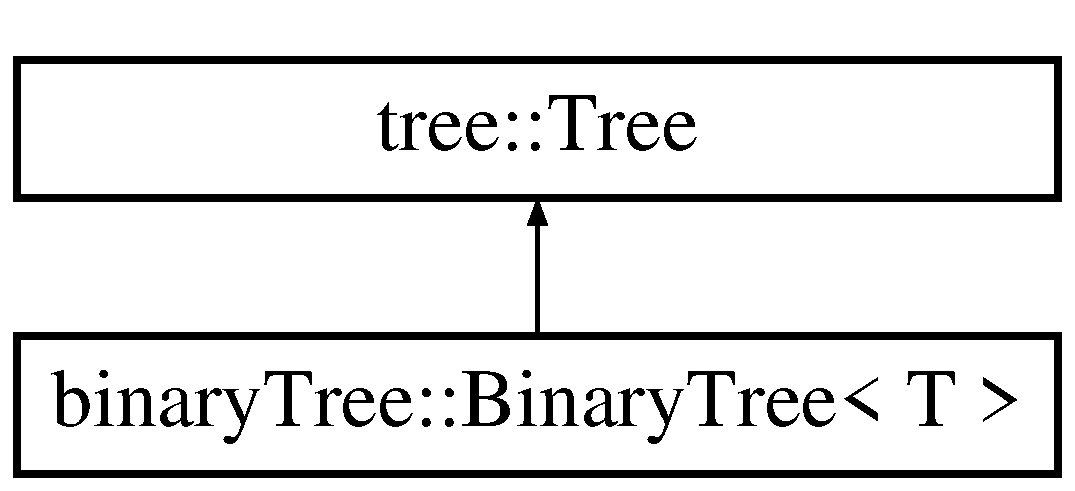
\includegraphics[height=2.000000cm]{classtree_1_1Tree}
\end{center}
\end{figure}
\subsection*{Protected Member Functions}
\begin{DoxyCompactItemize}
\item 
\hyperlink{classtree_1_1Tree_a66755a8dbcf714aa93e63952bdb62484}{Tree} ()
\begin{DoxyCompactList}\small\item\em Default Constructor\-: \end{DoxyCompactList}\item 
\hyperlink{classtree_1_1Tree_af393c36d4a1520937a7d5fcd985d9e08}{$\sim$\-Tree} ()
\begin{DoxyCompactList}\small\item\em Deconstructor\-: \end{DoxyCompactList}\item 
virtual void \hyperlink{classtree_1_1Tree_ae5b70de2d45be21d9b1b272c945b6248}{print} ()=0
\begin{DoxyCompactList}\small\item\em Pure virtual Print\-: \end{DoxyCompactList}\end{DoxyCompactItemize}
\subsection*{Protected Attributes}
\begin{DoxyCompactItemize}
\item 
int \hyperlink{classtree_1_1Tree_ae808b4b4b204faaa40e1e636ebfab8e6}{depth}
\begin{DoxyCompactList}\small\item\em \hyperlink{classtree_1_1Tree}{Tree} Depth. \end{DoxyCompactList}\end{DoxyCompactItemize}


\subsection{Detailed Description}
\hyperlink{classtree_1_1Tree}{Tree} Class\-: 

Definition at line 32 of file Tree.\-hpp.



\subsection{Constructor \& Destructor Documentation}
\hypertarget{classtree_1_1Tree_a66755a8dbcf714aa93e63952bdb62484}{\index{tree\-::\-Tree@{tree\-::\-Tree}!Tree@{Tree}}
\index{Tree@{Tree}!tree::Tree@{tree\-::\-Tree}}
\subsubsection[{Tree}]{\setlength{\rightskip}{0pt plus 5cm}tree\-::\-Tree\-::\-Tree (
\begin{DoxyParamCaption}
{}
\end{DoxyParamCaption}
)\hspace{0.3cm}{\ttfamily [protected]}}}\label{classtree_1_1Tree_a66755a8dbcf714aa93e63952bdb62484}


Default Constructor\-: 



Definition at line 50 of file Tree.\-hpp.

\hypertarget{classtree_1_1Tree_af393c36d4a1520937a7d5fcd985d9e08}{\index{tree\-::\-Tree@{tree\-::\-Tree}!$\sim$\-Tree@{$\sim$\-Tree}}
\index{$\sim$\-Tree@{$\sim$\-Tree}!tree::Tree@{tree\-::\-Tree}}
\subsubsection[{$\sim$\-Tree}]{\setlength{\rightskip}{0pt plus 5cm}tree\-::\-Tree\-::$\sim$\-Tree (
\begin{DoxyParamCaption}
{}
\end{DoxyParamCaption}
)\hspace{0.3cm}{\ttfamily [protected]}}}\label{classtree_1_1Tree_af393c36d4a1520937a7d5fcd985d9e08}


Deconstructor\-: 



Definition at line 55 of file Tree.\-hpp.



\subsection{Member Function Documentation}
\hypertarget{classtree_1_1Tree_ae5b70de2d45be21d9b1b272c945b6248}{\index{tree\-::\-Tree@{tree\-::\-Tree}!print@{print}}
\index{print@{print}!tree::Tree@{tree\-::\-Tree}}
\subsubsection[{print}]{\setlength{\rightskip}{0pt plus 5cm}virtual void tree\-::\-Tree\-::print (
\begin{DoxyParamCaption}
{}
\end{DoxyParamCaption}
)\hspace{0.3cm}{\ttfamily [protected]}, {\ttfamily [pure virtual]}}}\label{classtree_1_1Tree_ae5b70de2d45be21d9b1b272c945b6248}


Pure virtual Print\-: 



Implemented in \hyperlink{classbinaryTree_1_1BinaryTree_ad57b6b69f944ae45262c635fb7cc3bdc}{binary\-Tree\-::\-Binary\-Tree$<$ T $>$}.



\subsection{Member Data Documentation}
\hypertarget{classtree_1_1Tree_ae808b4b4b204faaa40e1e636ebfab8e6}{\index{tree\-::\-Tree@{tree\-::\-Tree}!depth@{depth}}
\index{depth@{depth}!tree::Tree@{tree\-::\-Tree}}
\subsubsection[{depth}]{\setlength{\rightskip}{0pt plus 5cm}int tree\-::\-Tree\-::depth\hspace{0.3cm}{\ttfamily [protected]}}}\label{classtree_1_1Tree_ae808b4b4b204faaa40e1e636ebfab8e6}


\hyperlink{classtree_1_1Tree}{Tree} Depth. 



Definition at line 46 of file Tree.\-hpp.



The documentation for this class was generated from the following file\-:\begin{DoxyCompactItemize}
\item 
lib/\-Data\-Structures/\hyperlink{Tree_8hpp}{Tree.\-hpp}\end{DoxyCompactItemize}

\chapter{File Documentation}
\hypertarget{BinaryTree_8hpp}{\section{lib/\-Data\-Structures/\-Binary\-Tree.hpp File Reference}
\label{BinaryTree_8hpp}\index{lib/\-Data\-Structures/\-Binary\-Tree.\-hpp@{lib/\-Data\-Structures/\-Binary\-Tree.\-hpp}}
}
{\ttfamily \#include \char`\"{}Tree.\-hpp\char`\"{}}\\*
{\ttfamily \#include $<$cstdlib$>$}\\*
{\ttfamily \#include $<$iostream$>$}\\*
\subsection*{Classes}
\begin{DoxyCompactItemize}
\item 
struct \hyperlink{structbinaryTree_1_1Node}{binary\-Tree\-::\-Node$<$ T $>$}
\begin{DoxyCompactList}\small\item\em Binary Tree \hyperlink{structbinaryTree_1_1Node}{Node}. \end{DoxyCompactList}\item 
class \hyperlink{classbinaryTree_1_1BinaryTree}{binary\-Tree\-::\-Binary\-Tree$<$ T $>$}
\begin{DoxyCompactList}\small\item\em Binary Tree class. \end{DoxyCompactList}\end{DoxyCompactItemize}
\subsection*{Namespaces}
\begin{DoxyCompactItemize}
\item 
\hyperlink{namespacebinaryTree}{binary\-Tree}
\begin{DoxyCompactList}\small\item\em \hyperlink{namespacebinaryTree}{binary\-Tree} Namespace \end{DoxyCompactList}\end{DoxyCompactItemize}
\subsection*{Constant Groups}
\begin{DoxyCompactItemize}
\item 
\hyperlink{namespacebinaryTree}{binary\-Tree}
\begin{DoxyCompactList}\small\item\em \hyperlink{namespacebinaryTree}{binary\-Tree} Namespace \end{DoxyCompactList}\end{DoxyCompactItemize}

\hypertarget{DoublyLinkedList_8hpp}{\section{lib/\-Data\-Structures/\-Doubly\-Linked\-List.hpp File Reference}
\label{DoublyLinkedList_8hpp}\index{lib/\-Data\-Structures/\-Doubly\-Linked\-List.\-hpp@{lib/\-Data\-Structures/\-Doubly\-Linked\-List.\-hpp}}
}
{\ttfamily \#include $<$cstdlib$>$}\\*
{\ttfamily \#include $<$iostream$>$}\\*
\subsection*{Classes}
\begin{DoxyCompactItemize}
\item 
struct \hyperlink{structdoublyLinkedList_1_1Node}{doubly\-Linked\-List\-::\-Node$<$ T $>$}
\item 
class \hyperlink{classdoublyLinkedList_1_1DoublyLinkedList}{doubly\-Linked\-List\-::\-Doubly\-Linked\-List$<$ T $>$}
\end{DoxyCompactItemize}
\subsection*{Namespaces}
\begin{DoxyCompactItemize}
\item 
\hyperlink{namespacedoublyLinkedList}{doubly\-Linked\-List}
\end{DoxyCompactItemize}
\subsection*{Constant Groups}
\begin{DoxyCompactItemize}
\item 
\hyperlink{namespacedoublyLinkedList}{doubly\-Linked\-List}
\end{DoxyCompactItemize}

\hypertarget{Matrix_8hpp}{\section{lib/\-Data\-Structures/\-Matrix.hpp File Reference}
\label{Matrix_8hpp}\index{lib/\-Data\-Structures/\-Matrix.\-hpp@{lib/\-Data\-Structures/\-Matrix.\-hpp}}
}
{\ttfamily \#include $<$stdexcept$>$}\\*
{\ttfamily \#include $<$iostream$>$}\\*
{\ttfamily \#include $<$string$>$}\\*
{\ttfamily \#include $<$vector$>$}\\*
{\ttfamily \#include $<$complex$>$}\\*
{\ttfamily \#include $<$initializer\-\_\-list$>$}\\*
\subsection*{Classes}
\begin{DoxyCompactItemize}
\item 
class \hyperlink{classmatrix_1_1Matrix}{matrix\-::\-Matrix$<$ T $>$}
\begin{DoxyCompactList}\small\item\em \hyperlink{classmatrix_1_1Matrix}{Matrix} class. \end{DoxyCompactList}\end{DoxyCompactItemize}
\subsection*{Namespaces}
\begin{DoxyCompactItemize}
\item 
\hyperlink{namespacematrix}{matrix}
\begin{DoxyCompactList}\small\item\em matrix Namespace \end{DoxyCompactList}\end{DoxyCompactItemize}
\subsection*{Constant Groups}
\begin{DoxyCompactItemize}
\item 
\hyperlink{namespacematrix}{matrix}
\begin{DoxyCompactList}\small\item\em matrix Namespace \end{DoxyCompactList}\end{DoxyCompactItemize}
\subsection*{Functions}
\begin{DoxyCompactItemize}
\item 
{\footnotesize template$<$typename T $>$ }\\std\-::ostream \& \hyperlink{namespacematrix_ab73e58c81eae2fdc97f26f72f31fe5ff}{matrix\-::operator$<$$<$} (std\-::ostream \&os, const Matrix$<$ T $>$ \&rhs)
\end{DoxyCompactItemize}
\subsection*{Variables}
\begin{DoxyCompactItemize}
\item 
const std\-::string \hyperlink{namespacematrix_a3410a3377815b8c5431e5436a31774c4}{matrix\-::empty\-Str} = std\-::string()
\begin{DoxyCompactList}\small\item\em Empty string used for default pad in matrix printing. \end{DoxyCompactList}\end{DoxyCompactItemize}

\hypertarget{SinglyLinkedList_8hpp}{\section{lib/\-Data\-Structures/\-Singly\-Linked\-List.hpp File Reference}
\label{SinglyLinkedList_8hpp}\index{lib/\-Data\-Structures/\-Singly\-Linked\-List.\-hpp@{lib/\-Data\-Structures/\-Singly\-Linked\-List.\-hpp}}
}
{\ttfamily \#include $<$cstdlib$>$}\\*
{\ttfamily \#include $<$iostream$>$}\\*
\subsection*{Classes}
\begin{DoxyCompactItemize}
\item 
struct \hyperlink{structsinglyLinkedList_1_1Node}{singly\-Linked\-List\-::\-Node$<$ T $>$}
\item 
class \hyperlink{classsinglyLinkedList_1_1SinglyLinkedList}{singly\-Linked\-List\-::\-Singly\-Linked\-List$<$ T $>$}
\end{DoxyCompactItemize}
\subsection*{Namespaces}
\begin{DoxyCompactItemize}
\item 
\hyperlink{namespacesinglyLinkedList}{singly\-Linked\-List}
\end{DoxyCompactItemize}
\subsection*{Constant Groups}
\begin{DoxyCompactItemize}
\item 
\hyperlink{namespacesinglyLinkedList}{singly\-Linked\-List}
\end{DoxyCompactItemize}

\hypertarget{Tree_8hpp}{\section{lib/\-Data\-Structures/\-Tree.hpp File Reference}
\label{Tree_8hpp}\index{lib/\-Data\-Structures/\-Tree.\-hpp@{lib/\-Data\-Structures/\-Tree.\-hpp}}
}
{\ttfamily \#include $<$cstdlib$>$}\\*
{\ttfamily \#include $<$iostream$>$}\\*
\subsection*{Classes}
\begin{DoxyCompactItemize}
\item 
class \hyperlink{classtree_1_1Tree}{tree\-::\-Tree}
\begin{DoxyCompactList}\small\item\em \hyperlink{classtree_1_1Tree}{Tree} Class\-: \end{DoxyCompactList}\end{DoxyCompactItemize}
\subsection*{Namespaces}
\begin{DoxyCompactItemize}
\item 
\hyperlink{namespacetree}{tree}
\begin{DoxyCompactList}\small\item\em Namespace\-: \end{DoxyCompactList}\end{DoxyCompactItemize}
\subsection*{Constant Groups}
\begin{DoxyCompactItemize}
\item 
\hyperlink{namespacetree}{tree}
\begin{DoxyCompactList}\small\item\em Namespace\-: \end{DoxyCompactList}\end{DoxyCompactItemize}

\hypertarget{SearchUtil_8cpp}{\section{lib/\-Searching/\-Search\-Util.cpp File Reference}
\label{SearchUtil_8cpp}\index{lib/\-Searching/\-Search\-Util.\-cpp@{lib/\-Searching/\-Search\-Util.\-cpp}}
}
{\ttfamily \#include \char`\"{}Search\-Util.\-h\char`\"{}}\\*
\subsection*{Namespaces}
\begin{DoxyCompactItemize}
\item 
\hyperlink{namespacesearchUtil}{search\-Util}
\begin{DoxyCompactList}\small\item\em \hyperlink{namespacesearchUtil}{search\-Util} Namespace \end{DoxyCompactList}\end{DoxyCompactItemize}
\subsection*{Constant Groups}
\begin{DoxyCompactItemize}
\item 
\hyperlink{namespacesearchUtil}{search\-Util}
\begin{DoxyCompactList}\small\item\em \hyperlink{namespacesearchUtil}{search\-Util} Namespace \end{DoxyCompactList}\end{DoxyCompactItemize}
\subsection*{Functions}
\begin{DoxyCompactItemize}
\item 
bool \hyperlink{namespacesearchUtil_abacab724882caea0ce2af75a7e208d41}{search\-Util\-::exists} ()
\end{DoxyCompactItemize}

\hypertarget{SearchUtil_8h}{\section{lib/\-Searching/\-Search\-Util.h File Reference}
\label{SearchUtil_8h}\index{lib/\-Searching/\-Search\-Util.\-h@{lib/\-Searching/\-Search\-Util.\-h}}
}
\subsection*{Namespaces}
\begin{DoxyCompactItemize}
\item 
\hyperlink{namespacesearchUtil}{search\-Util}
\begin{DoxyCompactList}\small\item\em \hyperlink{namespacesearchUtil}{search\-Util} Namespace \end{DoxyCompactList}\end{DoxyCompactItemize}
\subsection*{Constant Groups}
\begin{DoxyCompactItemize}
\item 
\hyperlink{namespacesearchUtil}{search\-Util}
\begin{DoxyCompactList}\small\item\em \hyperlink{namespacesearchUtil}{search\-Util} Namespace \end{DoxyCompactList}\end{DoxyCompactItemize}
\subsection*{Functions}
\begin{DoxyCompactItemize}
\item 
bool \hyperlink{namespacesearchUtil_abacab724882caea0ce2af75a7e208d41}{search\-Util\-::exists} ()
\end{DoxyCompactItemize}

\hypertarget{BogoSort_8hpp}{\section{lib/\-Sorting/\-Bogo\-Sort.hpp File Reference}
\label{BogoSort_8hpp}\index{lib/\-Sorting/\-Bogo\-Sort.\-hpp@{lib/\-Sorting/\-Bogo\-Sort.\-hpp}}
}
{\ttfamily \#include $<$vector$>$}\\*
{\ttfamily \#include $<$iostream$>$}\\*
{\ttfamily \#include $<$algorithm$>$}\\*
{\ttfamily \#include $<$stdlib.\-h$>$}\\*
\subsection*{Classes}
\begin{DoxyCompactItemize}
\item 
class \hyperlink{classBogoSort}{Bogo\-Sort$<$ T $>$}
\end{DoxyCompactItemize}

\hypertarget{StringUtil_8cpp}{\section{lib/\-String\-Util/\-String\-Util.cpp File Reference}
\label{StringUtil_8cpp}\index{lib/\-String\-Util/\-String\-Util.\-cpp@{lib/\-String\-Util/\-String\-Util.\-cpp}}
}
{\ttfamily \#include \char`\"{}String\-Util.\-h\char`\"{}}\\*
{\ttfamily \#include $<$string$>$}\\*
{\ttfamily \#include $<$iostream$>$}\\*
\subsection*{Namespaces}
\begin{DoxyCompactItemize}
\item 
\hyperlink{namespacestringUtil}{string\-Util}
\begin{DoxyCompactList}\small\item\em \hyperlink{namespacestringUtil}{string\-Util} Namespace \end{DoxyCompactList}\end{DoxyCompactItemize}
\subsection*{Constant Groups}
\begin{DoxyCompactItemize}
\item 
\hyperlink{namespacestringUtil}{string\-Util}
\begin{DoxyCompactList}\small\item\em \hyperlink{namespacestringUtil}{string\-Util} Namespace \end{DoxyCompactList}\end{DoxyCompactItemize}
\subsection*{Functions}
\begin{DoxyCompactItemize}
\item 
int \hyperlink{namespacestringUtil_a252b8681c024b4e02c792399e23c4469}{string\-Util\-::length} (const std\-::string \&in\-Str)
\begin{DoxyCompactList}\small\item\em Returns length of a string. \end{DoxyCompactList}\end{DoxyCompactItemize}

\hypertarget{StringUtil_8h}{\section{lib/\-String\-Util/\-String\-Util.h File Reference}
\label{StringUtil_8h}\index{lib/\-String\-Util/\-String\-Util.\-h@{lib/\-String\-Util/\-String\-Util.\-h}}
}
{\ttfamily \#include $<$sstream$>$}\\*
{\ttfamily \#include $<$string$>$}\\*
\subsection*{Namespaces}
\begin{DoxyCompactItemize}
\item 
\hyperlink{namespacestringUtil}{string\-Util}
\begin{DoxyCompactList}\small\item\em \hyperlink{namespacestringUtil}{string\-Util} Namespace \end{DoxyCompactList}\end{DoxyCompactItemize}
\subsection*{Constant Groups}
\begin{DoxyCompactItemize}
\item 
\hyperlink{namespacestringUtil}{string\-Util}
\begin{DoxyCompactList}\small\item\em \hyperlink{namespacestringUtil}{string\-Util} Namespace \end{DoxyCompactList}\end{DoxyCompactItemize}
\subsection*{Functions}
\begin{DoxyCompactItemize}
\item 
{\footnotesize template$<$typename T $>$ }\\std\-::string \hyperlink{namespacestringUtil_afdcf72298d021f62dac0e7d8fc4da881}{string\-Util\-::to\-String} (T in\-Var)
\begin{DoxyCompactList}\small\item\em Prints any type to string. \end{DoxyCompactList}\item 
int \hyperlink{namespacestringUtil_a252b8681c024b4e02c792399e23c4469}{string\-Util\-::length} (const std\-::string \&in\-Str)
\begin{DoxyCompactList}\small\item\em Returns length of a string. \end{DoxyCompactList}\end{DoxyCompactItemize}

%--- End generated contents ---

% Index
\newpage
\phantomsection
\addcontentsline{toc}{part}{Index}
\printindex

\end{document}
